% scopiazzato dal template di Matteo Longeri (grazie!)
%%%%%%%%%%%%%%%%%%%%%%%%%%%%%%%%%%%%%%%%%%%%%%%%%%%%%%
\documentclass[a4paper]{report}
% o article, book, ...



%%%%%%%%%%%%%%%%%%%%%%%%%%%%%%%%%%%%%%%%%%%%%%%%%%%%%%
% packages...
\usepackage[utf8]{inputenc}
\usepackage[english,italian]{babel}
\usepackage[hyphens]{url}

% Per generare il file PDF aderente alle specifiche PDF/A-1b. Verificarne poi la validità.
%\usepackage[a-1b]{pdfx}

\usepackage{hyperref}
\usepackage{graphicx}
\graphicspath{ {./img/} }


% Per inserire testo a caso in attesa di realizzare i capitoli
\usepackage{lipsum}

% Package per mantenere le immagini presenti nel documento all'interno delle sezioni di appartenenza
\usepackage[section]{placeins}

%%%%%%%%%%%%%%%%%%%%%%%%%%%%%%%%%%%%%%%%%%%%%%%%%%%%%
\begin{document}

% Frontespizio
\begin{titlepage}
\begin{center}

\includegraphics[width=\textwidth]{Logo.jpg}\\
{\large{\bf Corso di Laurea Triennale in Informatica}}
\end{center}
\vspace{12mm}
\begin{center}
{\huge{\bf TITOLO}}\\
\vspace{4mm}
{\huge{\bf TITOLO}}\\
\vspace{4mm}
{\huge{\bf TITOLO}}\\
\end{center}
\vspace{12mm}
\begin{flushright}
{\large{\bf Tesi di Laurea di:}}\\
{\large{\bf Marco Belotti}}\\
{\large{\bf Matr. 871440}}\\
\end{flushright}
\vspace{4mm}
\begin{flushleft}
{\large{\bf Relatore:}}\\
{\large{\bf Andrea Trentini}}\\
\vspace{4mm}
%{\large{\bf Correlatore:}}\\
%{\large{\bf CORREL}}\\
\end{flushleft}
\vspace{12mm}
\begin{center}
{\large{\bf Anno Accademico 2019/2020}}
\end{center}
\end{titlepage}


\tableofcontents


\chapter{Introduzione}
L'inquinamento atmosferico è un tema che viene spesso discusso e dibattuto, visto che respirare un'aria pulita è considerato un requisito basilare per la buona salute umana. Da anni il WHO\cite{world2006air} si occupa di studiare i potenziali effetti dell'inquinamento sulla salute umana, cercando di stimare che tipo di impatto possa avere un'esposizione prolungata ad alte concentrazioni.  

Chiaramente non è facile riuscire a stabilire con certezza il collegamento tra causa (esposizione agli inquinanti) ed effetto (malattie e morte) poichè spesso i danni si manifestano solo a seguito di ripetute e prolungate esposizioni, così come non è facile riuscire a stabilire con certezza che una morte sia stata causata esplicitamente dall'inquinamento atmosferico.  

L'inquinamento atmosferico è un fenomeno molto complicato da analizzare, poichè sia per quanto riguarda la produzione e l'emissione in atmosfera che per la dispersione entrano in gioco molti fenomeni e fattori, che hanno scale spaziali molto differenti e che è difficile riuscire ad analizzare correttamente.  

Se in alcune zone del mondo, soprattutto quelle dei paesi in forte via di sviluppo come il sud-est asiatico o l'India, l'inquinamento rappresenta ancora un problema molto grave causato dall'aumento del fabbisogno energetico che è stato soddisfatto incrementando l'uso di combusitibili fossili, in Europa (come in altre parti del mondo) negli ultimi 25 anni si è registrato un disaccoppiamento tra la crescita economica e le emissioni dei principali inquinanti, causato da un maggiore impegno nel loro contenimento da parte dei governi, che hanno imposto limitazioni e misure sempre più stringenti.\cite{cattani2014analisi}  

È quindi normale che sia la comunità scientifica che le autorità incaricate di decidere le misure di contenimento da mettere in campo siano interessate a capire quale sia il reale andamento delle concentrazioni di inquinanti, cercando di identificare quali possano essere i metodi più efficaci e quanto le variazioni registrate siano attribuibili specificatamemente ai cambiamenti delle emissioni umane rispetto agli effetti di altri fattori come il clima che possono avere un'influenza molto maggiore sulle concentrazioni registrate.\cite{porter2001ozone}  

Quasi tutti gli inquinanti di maggior interesse, come gli ossidi di azoto, il biossido di zolfo, il monossido di carbonio, il particolato e l'ozono sono infatti caratterizzati da una forte variabilità stagionale che, per esempio, non ci permette di confrontare valori registrati durante la stagione estiva con quelli invernali, così come l'azione di agenti atmosferici come il vento e la pioggia possono portare ad abbattimenti delle concentrazioni. Nella pianura padana, per esempio, è infatti frequente assistere, specialmente nei mesi invernali che sono già quelli più critici per le concentrazioni di molti inquinanti, a lunghi periodi senza precipitazioni che portano a grossi aumenti delle concentrazioni, che però vengono rapidamente abbattute all'arrivo della pioggia. %RIVEDI  

Per poter quindi trarre delle conclusioni oggettive sullo stato della qualità dell'aria, riuscendo ad identificare le cause delle variazioni che si registrano e quindi a capire anche l'efficacia delle misure prese, nel corso degli ultimi anni molti studi si sono avvalsi di diverse tecniche statistiche/probabilistiche per poter fare un'analisi oggettiva dell'inquinamento atmosferico.\cite{cattani2014analisi}\cite{rao1994detecting}\cite{libiseller2005meteorological}\cite{pbl2010trends}

Riuscire ad avere a disposizione tecniche e modelli che ci permettono di analizzare l'andamento delle concentrazioni e ad identificare le cause che possono cambiare questo andamento ci permette di capire quali siano le aree più critiche su cui andare ad intervenire ma ci può anche permettere di identificare gli interventi più efficaci e sui quali conviene investire maggiormente. La crescita economica e l'aumento del fabbisogno energetico rendono quindi fondamentale il controllo delle emissioni, per poter mantenere la qualità dell'aria a livelli non pericolosi per la salute umana e al tempo stesso non bloccare le attività economiche.  

Qualsiasi studio sui trend degli inquinanti, così come qualsiasi conclusione che ne può derivare, non possono quindi non tener conto degli effetti della meteorologia sulle concentrazioni, poichè i risultati che si otterrebbero correrebbero il rischio di non rappresentare il cambiamento nelle emissioni antropiche ma anche una variazione nei fenomeni atmosferici e negli agenti climatici.  

Il nostro obbiettivo è quindi stato quello di ricercare una tecnica per normalizzare i dati sull'inquinamento rispetto alla meteorologia e al clima, ovvero che fosse in grado di eliminare l'influenza degli agenti atmosferici come pioggia, vento e radiazione solare e della stagionalità che porta ad avere condizioni più o meno favorevoli alla dispresione dalle concentrazioni registrate degli inquinanti, in modo da arrivare poi ad avere una serie storica su cui poter fare analisi sull'efficacia delle misure prese nel corso degli anni per il contenimento delle concentrazioni.  

Un metodo comune per riuscire a fare questa "pulizia" dei dati si basa sulla creazione di modelli statistici che tramite l'uso di diverse variabili predittrici, come le misure meteorologiche su vento, precipitazioni e radiazione solare e variabili temporali legate al giorno dell'anno e alla date, cercando di prevedere quale potrebbe essere la concentrazione registrata di un inquinante. Se i modelli che riusciamo a creare si rivelano abbastanza precisi nell'attività predittoria e in grado di spiegare buona parte della varianza delle concentrazioni allora possiamo usarli con una certa confidenza per eliminare gli effetti della meteorologia dalle concentrazioni di inquinanti.  

Questo procedimento viene però complicato dal fatto che le dinamiche che portano la meteorologia a modificare le concentrazioni varino molto a seconda della località e che quindi differenti contesti, come ad esempio possono essere una città rispetto ad una località montana o situata a fondo valle, necessitino trattazione specifiche a seconda del caso. Inoltre è chiaro come le variabili meteorologiche tra di loro siano collegate e correlate e questo porta all'insorgere di una serie di problemi come la normalità, la multi collinearità e l'indipendenza che rendono la trattazione con diversi metodi molto difficile e complicata.  

Nel corso degli ultimi tre decenni nel mondo dell'informatica ha preso campo un'area detta machine learning (ML), che fa uso dei computer e della statistica per creare dei modelli predittori che potessero porsi come alternativa ai classici metodi statistici già esistenti. Sono quindi state sviluppate tecniche di ML non parametriche che, grazie all'uso dei computer per analizzare grosse moli di dati, permettono di arrivare alla creazione di modelli con buone capacità predittive anche senza occuparsi dei problemi che invece caratterizzano gli approcci puramente statistici.  

ARPA Lombardia possiede, sul territorio regionale, una rete di 85 stazioni fisse che, per mezzo di analizatori automatici, sono in grad di fornire rilevazioni ad intervalli di tempo regolari, permettendoci di creare quindi un dettagliato catalogo dei valori delle concentrazioni nel corso del tempo. Tutte queste rilevazioni vengono poi rese accessibili liberamente tramite archivi online, per permetterne la libera consultazione da parte di tutti i cittadini.  

Nel nostro studio abbiamo quindi fatto uso di questi dati, unitamente a quelli delle variabili meteorologiche sempre resi disponibili da ARPA Lombardia, per creare tramite l'uso di una tecnica di machine learning chiamata random forest dei modelli predittivi che ci permettano di arrivare a fare questa normalizzazione delle concentrazioni di inquinanti rispetto alla meteorologia e quindi di anlizzare come si sia evoluta la situazione nella nostra regione nel corso degli anni dal 2012 ad oggi, cercando di capire quali siano stati i provvedimenti e gli eventi più efficaci nell'abbattimento delle concentrazioni.  

Nel capitolo 2 viene introdotto random forest e viene mostrato come questa tecnica possa esssere utilizzata per eliminare gli effetti della meteorologia e della stagionalità dall'andamento delle concentrazioni.  

Nel capitolo 3 viene analizzata, utilizzando la tecnica appena discussa, la situazione regionale andando a controllare l'andamento delle serie dei principali inquinanti nei capoluoghi di provincia lombardi.  

Nel capitolo 4 verranno presentate le analisi svolte sull'influenza del traffico sulle concentrazioni di tre inquinanti: ossidi di azoto, particolato atmosferico (PM10 e PM2.5) e monossido di carbonio.  
Nel capitolo 5 verrà presentata un'analisi del periodo di diffusione dell'epidemia di Covid-19 e di quali siano stati gli effetti del conseguente lockdown svoltosi nei mesi di marzo ed aprile sulle concentrazioni.

\chapter{Normalizzazione meteorologica utilizzando Random Forest}
L'atmosfera è lo strato gassoso che ricopre esternamente la terra come un involucro ed è costituita principalmente da azoto e ossigeno, mescolati con piccole quantità di altri gas e pulviscolo. La porzione più bassa, che sta a diretto contatto col suolo, è definita strato limite planetario (Planetary Boundary Layer, o PBL, in inglese) e sia la sua struttura che l'evoluzione hanno influenze fondamentali sul comportamento degli inquinanti atmosferici di maggior interesse.\cite{dina2009concentrazione}  

A causa della sua struttura, infatti, gli inquinanti emessi in atmosfera rimangono bloccati al suo interno e variazioni sull'altezza, che può variare da qualche centinaio di metri a qualche chilometro, causate da agenti atmosferici come il vento, la temperatura e la pressione atmosferica, hanno l'effetto di disperdere o aumentare le concentrazioni di tali inquinanti.\cite{stull2012introduction}  

La forte variabilità stagionale che si riscontra su tanti inquinanti è infatti direttamente collegata al fatto che nei mesi invernali (così come nelle ore notturne) l'altezza dello strato di rimescolamento sia ridotta e porti quindi ad un aumento delle concentrazioni.  

Per poter analizzare i dati sull'inquinamento atmosferico volendo capire come le misure messe in atto e le attività antropiche abbiano influenzato l'andamento delle concentrazioni nel corso degli anni non possiamo trascurare questa grossa influenza da parte della meteorologia e del clima, altrimenti non sarebbe possibile stabilire con certezza quanta influenza possa avere avuto un determinato provvedimento rispetto a quella data dalla variazione delle condizioni atmosferiche.  

Nel corso degli anni diversi studi hanno provato ad affrontare la questione usando metodi che portassero ad ottenere dei modelli statistici in grado di capire e modellare le relazioni tra inquinanti e condizioni atmosferiche e, indipendentemente dal metodo usato, si è visto come variabili legate alla meteorologia, all'altezza dello strato di rimescolamento ed alla stagionalità siano in grado di spiegare con una certa precisioni gli andamenti delle serie di inquinanti. \cite{aldrin2005generalised}\cite{elminir2005depndence}\cite{eagleman1991air}\cite{seagal1982numerical}\cite{cattani2014analisi}\cite{barmpadimos2011influence}  

I processi atmosferici, però, sono molto complessi, non lineari e spesso si riscontra collinearità tra le osservazioni di variabili diverse, una situazione in cui i valori di una possono essere approssimati in modo preciso da quelli di un'altra, e questo rende la modellazione grazie all'uso di metodi parametrici, cioè quelli basati su metodi puramente matematici come la regressione lineare, molto complicata poichè questi fattori influiscono molto sulla precisione e sull'affidabilità dei risultati ottenuti.   

Il machine learning, grazie all'uso di metodi non parametrici, ovvero metodi che non hanno bisogno di fare nessun tipo di assunzione sui dati considerati o sulle relazioni che intercorrono tra le diverse variabili, che quindi si adattano perfettamente ad un'analisi così complessa come quella degli inquinanti e della loro dispersione in atmosfera, ci permette di arrivare ad estrarre dei modelli in grado di simulare in modo abbstanza preciso le relazioni tra le diverse variabili in gioco.  

Una volta in possesso di uno strumento che sappia spiegarci come variazioni dei valori di una variabile influenzino quelli di un'altra, che nel nostro caso significa arrivare ad ottenere un modello capace di dirci come cambiamenti nelle condizioni atmosferiche e nella stagionalità portino a cambiare le concentrazioni registrate per gli inquinanti, diventa semplice anche arrivare ad eliminare la loro influenza. Le variabili predittrici, ovvero quelle delle quali vogliamo capire ed eliminare l'influenza dalle concentrazioni degli inquinanti, utilizzate nei nostri modelli sono state: la temperatura, le precipitazioni registrate, il numero di giorni passati dalle ultime precipitazioni, l'umidità relativa, la radiazione globale e direzione e velocità del vento. Inoltre sono state inserite anche il giorno dell'anno ed il giorno della settimana, due variabili temporali che potessero fare da proxy per gli andamenti tipici stagionali e settimanali (dovute alle maggiori attività antropiche, soprattutto nelle città, durante i giorni feriali) mostrati dalle concentrazioni di molti inquinanti. 

Analizzando la serie di ogni inquinante e riportandola, grazie all'uso di un modello appositamente costruito basandosi sui dati di tale serie, a condizioni meteorologiche e di stagionalità uguali per tutti i giorni possiamo quindi arrivare ad ottenere una serie il cui andamento sia indipendente dall'influenza data da questi fattori.

I metodi non parametrici esistenti nel campo del machine learning adatti ad affrontare problemi di regressione, ovvero problemi in cui vogliamo fare previsioni su una quantità numerica, come nel nostro caso vogliamo fare per le concentrazioni degli inquinanti, partendo dai valori di altre grandezze (le variabili meteorologiche e stagionali nel nostro caso), sono diversi ed ognuno è più adatto ad affrontare determinati problemi rispetto ad altri. Noi abbiamo scelto di utilizzare Random Forest, un metodo d'insieme basato sull'uso di molteplici alberi di decisione, inventato da Leo Breiman nel 2001.\cite{breiman2001random}

Gli alberi di decisione sono strutture usate per fare previsioni in cui, partendo dalla radice, si scende verso le foglie attraversando una serie di nodi intermedi contenenti una condizione che ci indicherà in quale sottoalbero proseguire la nostra discesa, fino ad arrivare alla foglia in cui sarà contenuto il risultato della previsione fatta dall'albero.  

Gli alberi di decisione sono una tecnica valida poichè non fanno nessun tipo di assunzione sulla struttura delle relazioni che sono presenti tra le diverse variabili utilizzate, così come permettono collinearità e sono capaci di scartare le misure che risultano irrilevanti rispetto alla variabile da predirre. In fase di costruzione, grazie all'uso di specifici algoritmi, questi alberi vengono creati in modo che le condizioni presenti nei nodi intermedi dell'albero, e che ci guidano verso il risultato della previsione, riescano a minimizzare il più possibile l'errore delle previsioni fatte dal modello sui dati usati in tale fase.

Queste strutture, specialmente se le si lascia crescere liberamente in profondità, soffrono molto di un problema detto overfitting, ovvero che i modelli ottenuti si adattono perfettamente ai dati utilizzati in fase di costruzione, ma quando poi si prova a verificare le loro prestazioni su dati nuovi risultano scarse, poichè le relazioni individuate dal modello risultano essere troppo contaminate da rumore presente in tali dati.\cite{bramer2007avoiding}

Random Forest, grazie all'uso di un numero elevato di alberi di decisione (da qui il termine forest), ciascuno costruito a partire da un sottoinsieme estratto casualmente dai dati iniziali, riesce a controllare il problema dell'overfitting mantenendo però tutti i vantaggi già presenti per gli alberi di decisione e che quindi lo rendono un algoritmo che si adatta perfettamente al tipo di lavoro che vogliamo fare. Random Forest, infatti, non fa nessun tipo di assunzione sulla struttura dei dati e delle relazioni che intercorrono tra ciascuna variabile, che è un grosso vantaggio quando stiamo trattando un problema complesso come quello della dispersione di inquinanti in atmosfera. È inoltre capace di selezionare in modo automatico le variabili più importanti, che poi userà maggiormente nell'attività predittoria, senza però porre vincoli nè sul numero di grandezze utilizzate nè su eventuali relazioni che possono intercorrere tra ciascuna. Random Forest ha inoltre il vantaggio di poter utilizzare contemporaneamente sia variabili numeriche che categoriche, senza richiedere particolari pre-trattazioni come invece avviene con altri metodi. 

Random Forest ci permette di analizzare come ogni modello operi per fare delle scelte, tramite strumenti come l'importanza delle variabili, che ci indica quali risultino più utilizzate ed influenti sulla precisione dei risultati ottenuti, o i partial dependence plots, che ci mostrano come i valori di una singola variabile influenzino le previsioni fatte dal modello. Questi sono strumenti molto utili perchè ci permettono di studiare, oltre ai risultati previsti dal modello, anche come ci si sia arrivati potendo così approfondire le relazioni e le dinamiche individuate.

Di ogni modello sono state valuate le prestazioni grazie all'uso della tecnica del validation set, una tecnica molto conosciuta che grazie all'utilizzo di una parte dei dati iniziali, che viene sottratta a quelli usati per creare il modello, permette di verificare quanto siano precise le previsioni fatte da un modello confrontandole con valori reali.  

L'algoritmo Random Forest permette di personalizzare alcuni aspetti del suo funzionamento per cercare di ottimizzarne le performance grazie all'uso di alcuni iperparametri, che vanno settati prima della creazione del modello e ne determinano le regole da applicare in tale fase. Una delle prime attività svolte, dopo aver verificato che fosse effettivamemte possibile utilizzare Random Forest per ottenere la normalizzazione meteorologica, è stata proprio una ricerca per individuare i valori migliori da assegnare ai diversi iperparametri in modo da ottenere il miglior compromesso possibile tra performance e prestazioni. Il numero di alberi creato in ciascuna foresta è stato di 300, la profondità massima di ogni singolo albero è stata fissata a 20 ed il numero di variabili da utilizzare per creare le condizioni presenti nei nodi intermedi a 5.

Ogni località ed ogni inquinante sono stati trattati con modelli specifici, costruiti di volta in volta utilizzando rilevazioni che potesssero rappresentare fedelmente le condizioni meteorologiche e di inquinamento di ogni posto considerato.  

Quello che abbiamo quindi ottenuto da Random Forest sono modelli che, ricevuta in ingresso una data ed i valori delle condizioni meteorologiche e atmosferiche, sono in grado di prevedere con una certa precisione quale sarebbe stata la concentrazione dell'inquinante misurata per quel giorno se si fossero verificate tali condizioni meteorologiche.  

Una volta in possesso di uno strumento di questo tipo diventa facile capire come eliminare l'influenza della meteorologia e delle condizioni atmosferiche dalle concentrazioni degli inquinanti, poichè, per ogni giorno della serie considerata, basta far fare al nostro modello molte previsioni, variando di volta in volta le condizioni atmosferiche, e poi calcolarne la media, che rappresenta quindi la concentrazione dell'inquinante per tale data se si fossero verificate condizioni medie. Per ottenere le serie utilizzate nelle nostre analisi per ogni giornata sono state fatte 1000 previsioni, variando di volta in volta i valori delle variabili predittrici, poichè si è visto che pur aumentando ulteriormente questo numero non si riuscisse ad ottenere risultati più precisi.

Ripetendo questo passaggio per tutti i giorni di una serie e per diversi inquinanti e località siamo così arrivati ad ottenere delle serie il cui andamento fosse stato "pulito" dall'influenza della meteorologia, permettendoci quindi di analizzarne meglio sia il trend che di verificare in modo più preciso quale sia stato l'impatto delle misure di contenimento prese.  

Fondamentale per il funzionamento della nostra tecnica era aver a disposizione molti dati, sia per quanto riguarda le serie delle concentrazioni di inquinante che per le variabili meteorologiche scelte. ARPA Lombardia, che da anni si occupa di monitoraggio dell'aria su tutto il territorio regionale, grazie alla sua vasta rete di rilevazione raccoglie tutte queste misure, che sono poi rese disponibili per il libero download da parte di chiunque. In assenza di questi dati non sarebbe possibile fare analisi di questo tipo, poichè per imparare le diverse relazioni tra le variabili in gioco i nostri modelli hanno per forza bisogno di grandi quantità di dati, che possano descrivere tutte le diverse situazioni riscontrabili nella realtà.

Tutto il lavoro di raccolta ed analisi dei dati è stato fatto utilizzando il linguaggio open source Python. Per l'utilizzo dell'algoritmo Random Forest ci si è appoggiati all'implementazione presente nella libreria Scikit-learn.\cite{scikit-learn}

\chapter{La situazione in Lombardia}
Inizialmente sono state affrontate una serie di analisi in cui, tramite l'applicazione di random forest per ottenere la normalizzazione dei dati sull'inquinamento relativamente alle condizioni meteorologiche, si è cercato di delinare il quadro della situazione per quanto riguarda i principali inquinanti atmosferici in Lombardia sfruttando i vantaggi derivanti dall'aver eliminato dalle concentrazioni l'influenza della meteorologia.

Sono state analizzate le serie storiche normalizzate dei principali inquinanti atmosferici, usando i dati registrati nei dodici capoluoghi di provincia lombardi. Per ogni inquinante di ogni capoluogo è stato creato un modello apposito, così da poter analizzare ogni situazione con un modello specifico creato appositamente per cercare di stimare al meglio le dinamiche locali degli eventi climatici e la loro relazione con gli inquinanti considerati. 

Il requisito di iniziare a considerare le serie storiche con cui creare i modelli solo a partire dalla data di messa in funzione del sensore più recente tra tutti quelli delle variabili coinvolte nella loro creazione ha purtroppo limitato il periodo considerato dalle nostre analisi, poichè per la maggior parte delle località le rilevazioni della direzione e velocità del vento, che è sicuramente uno dei fattori più influenti sull'andamento delle concentrazioni, sono iniziate solo nell'ultimo decennio.Una possibile soluzione a questo problema poteva essere quella di usare i valori medi di ciascuna variabile per il periodo in cui non fossero disponibili le registrazioni, ma questo, specialmente se fatto su periodi estesi, portava di fatto ad alterare le prestazioni e l'affidabilità del nostro modello poichè causava l'introduzione di un numero consistente di dati "fittizzi" che compromettevano l'individuazione delle diverse dinamiche che governano gli andamenti delle concentrazioni.

I modelli ottenuti nel corso delle analisi hanno avuto tutti prestazioni molto buone, specialmente quelli relativi all'ozono, con le polveri sottili che invece si sono rivelate l'inquinante con cui fanno più fatica ad adattarsi, evidenziando come per questo tipo di inquinanti, che arrivano a percorrere anche grosse distanze, le sole variabili delle rilevazioni meteorologiche di superfice e temporali considerate non siano sufficienti per spiegarne completamente l'andamento, che è governato da eventi su scale molto più grandi di quelle descritte dalle nostre variabili. 

Come si può osservare in figura\ref{fig:importanza_tot}, tra tutti i modelli ottenuti la variabile più importante è risultata essere la temperatura, seguita dalla data e dal giorno dell'anno. Questa considerazione però non dovrebbe meravigliarci se pensiamo al collegamento che esiste tra ciascuna e l'inquinamento: la temperatura serve sia ad identificare i cicli stagionali che eventuali periodi più caldi o freddi della media in cui la gente potrebbe inquinare maggiormente in risposta a questi eventi, la data ci permette di identificare l'evoluzione nel corso degli anni dei valori registrati, e quindi la presenza di eventuali trend o andamenti particolari, e il giorno dell'anno serve per identificare la stagionalità caratteristica degli inquinanti.  
Alle variabili legate alle precipitazioni, ovvero la quantità registrata e il numero di giorni trascorsi dall'ultimo evento, è sempre stata assegnata un'importanza abbastanza bassa. È bene ricordare, però, che l'importanza delle variabili è calcolata come il totale della diminuzione dell'impurità dei nodi della foresta, pesata per la probabilità di raggiungere ciascun nodo. Questa è quindi una misura che cerca di stimare come il nostro modello lavori per fare le previsioni, ma non indica assoultamente che tipo di relazioni ci siano tra la variabile considerata e quella da predirre. Quindi, anche se nei nostro modelli alle precipitazioni viene associata una bassa importanza, non significa che non abbiano influenza sulle concentrazioni registrate, ma semplicemente che la variabile per lui è meno utile nel fare previsioni più precise. 

\begin{figure}[h]
\centering
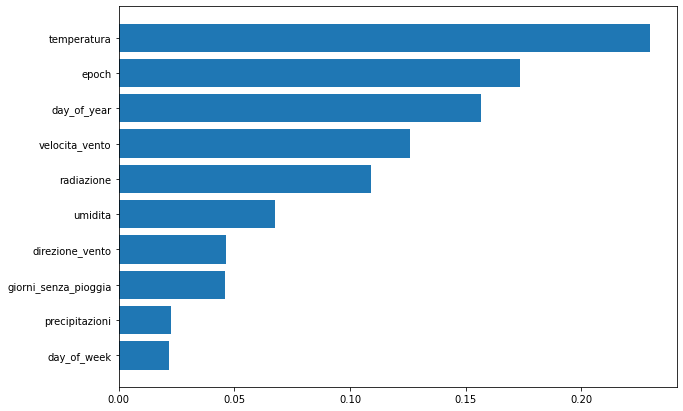
\includegraphics[width=0.75\textwidth]{intro_importanza_totale}
\caption{Media delle importanze delle variabili predittrici nei modelli generati durante le nostre analisi}
\label{fig:importanza_tot}
\end{figure}

\section{$NO_x$ e $NO_2$}
Nella categoria degli ossidi di azoto sono considerati due inquinanti di diverso interesse e che quindi è bene analizzare separatamente. Il monossido di azoto, infatti, alle concentrazioni tipiche misurate non risulta pericoloso nè per la salute umana nè per la vegetazione; il biossido di azoto, invece, desta sicuramente una maggior preoccupazione per i suoi effetti sulla salute. Per questo motivo sono state considerate ed analizzate separatamente le serie dei sensori misuratori di $NO_x$ e di quelli dedicati solo al biossido.

Inizialmente sono state analizzate le serie degli ossidi di azoto. Quando si considerano questi inquinanti è bene ricordare che il monossido ha principalmente origine primaria, mentre il biossido si genera in atmosfera grazie all'ossidazione del primo e quindi ha origine principalmente secondaria. All'emissione, infatti, si stima che il biossido sia circa il 5/10\% del totale per questa categoria.\cite{arpa2018rapporto}  
Entrambi sono emessi in atmosfera da processi di combustione ad alta temperatura (impianti di riscaldamento, motori dei veicoli, combustioni industriali, centrali di potenza, ecc..) e per ossidazione dell'azoto presente in atmosfera (o dei suoi composti contenuti nei combustibili utilizzati). Il biossido di azoto, oltre che alla pericolosità per quanto riguarda la salute di persone e vegetazione, ha un ruolo fondamentale nella formazione dello smog fotochimico in quanto è l'intermediario per la produzione di inquinanti secondari come l'ozono.

Secondo l'inventario regionale INEMAR 2017\cite{inemar2017} la categoria maggiormente responsabile per le emissioni di questi inquinanti è il trasporto su strada, con un contributo pari al 50\% del totale delle emissioni, seguita dalle combustioni industriali e civili (con circa il 15\% di contributo ciascuna). Sempre secondo l'inventario il combustibile maggiormente responsabile delle emissioni di questa categoria è il diesel, con oltre il 50\% del totale delle emissioni, seguito dal gas naturale (20\%).

Le prime normative introdotte per contenerne le concentrazioni sono arrivate nei primi anni 90, imponendo limiti alle emissioni degli impianti e favorendo l'uso del gas naturale al posto di gasolio e cherosene come combustibili. Negli anni più recenti i limiti normativi sono stati ulteriormente abbassati. Per quanto riguarda il traffico, visto che è il settore maggiormente responsabile, i provvedimenti più importanti sono sicuramente l'introduzione delle marmitte catalitiche e l'introduzione di limiti alle emissioni dei veicoli, con le famose categorie EuroX. Proprio questo ultimo aspetto ha fatto sì che, sebbene nel corso degli anni il numero dei veicoli circolanti e dei kilometri percorsi sia aumentato, l'inquinante abbia comunque fatto registrare un trend in forte calo nel corso degli anni\cite{iir2020}.

Nei modelli ottenuti le variabili più importanti sono state la temperatura, che è risultata quella col valore decisamente maggiore rispetto alle altre, il giorno dell'anno e la velocità del vento. Sicuramente non siamo sorpresi dalle prime due, visto il classico andamento stagionale dell'inquinante, legato sia alle maggiori emissioni antropiche durante il periodo invernale che alle condizioni atmosferiche più sfavorevoli alla dispersione. Anche il vento, specialmente la sua velocità, è risultato un buon predittore per le concentrazioni di ossidi di azoto, non sorprendentemente vista la forte azione dispersiva legata a questo fattore.

\begin{figure}[h]
\centering
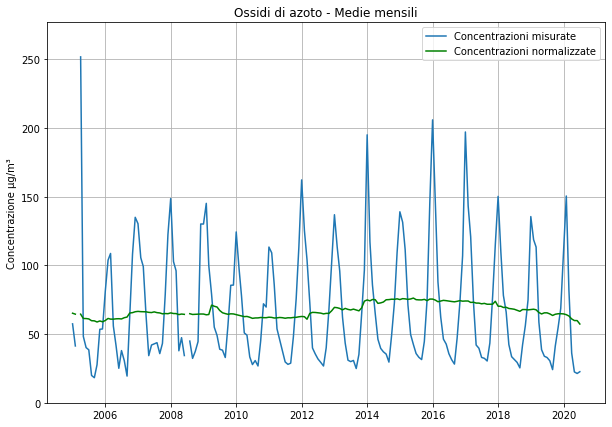
\includegraphics[width=0.75\textwidth]{nox_medie_mensili}
\caption{Confronto tra le medie mensili delle serie storiche rilevate dai sensori e quelle delle serie normalizzate}
\label{fig:nox_medie_mensili}
\end{figure}

\begin{figure}[h]
\centering
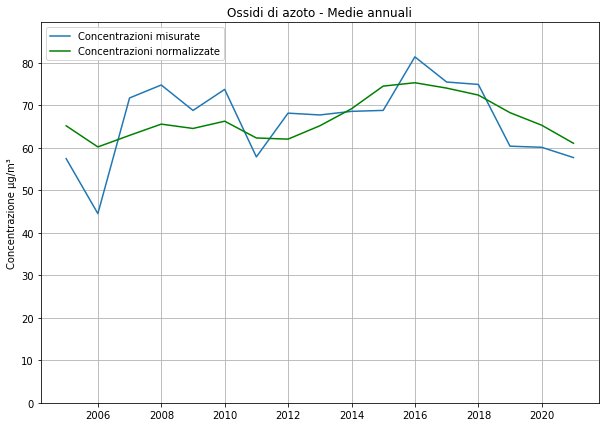
\includegraphics[width=0.75\textwidth]{nox_medie_annuali}
\caption{Confronto tra le medie annuali delle serie storiche rilevate dai sensori e quelle delle serie normalizzate}
\label{fig:nox_medie_annuali}
\end{figure}

Controllando il grafico in figura\ref{fig:nox_medie_mensili} delle medie mensili si nota come la serie normalizzata riesca a non essere influenzata dall'andamento stagionale, mantenendo sempre un livello "medio" costante, che è proprio il risultato che ci aspettavamo di ottenere dall'applicazione della nostra tecnica. Noi volevamo riuscire ad avere delle serie che fossero indipendenti da tutti questi fattori che possono incidere sulle concentrazioni e visto l'andamento mostrato da quella ottenuta, che rimane approssimativamente intorno ad un valore "medio" indipendentemente dalla giornata, possiamo essere abbastanza fiduciosi di essere riusciti a stimarla con una buona precisione.
Sulle medie annuali, riportate in figura\ref{fig:nox_medie_annuali} vengono sicuramente eliminati i picchi, probabilmente causati da condizioni meteorologiche più favorevoli/sfavorevoli all'accumulo avute da alcuni anni in particolare (ad esempio 2006 o 2011), ma l'andamento delle due serie risulta comunque compatibile, ancora una volta a dimostrazione della validità del risultato ottenuto, che sarebbe sicuramente stata messa in discussione se si fossero ottenuti dei risultati completamente diversi.

Guardando i grafici si vede chiaramente che l'andamento delle concentrazioni misurate dal 2006 ad oggi sia abbastanza costante, con un aumento di circa $10\mu g/m^3$ registrato tra gli anni 2012 e 2016, seguito però poi da un costante calo che ormai le ha riportate ai livelli di 8 anni fa. Se avessimo avuto a disposizione le serie complete a partire dai primi anni 90 sicuramente avremmo visto un trend negativo nelle concentrazioni, poichè è stato proprio in quel decennio che le emissioni sono state maggiormente ridotte. Negli ultimi anni non sono state introdotte nuove importanti normative a riguardo, se non aggiornamenti dei limiti imposte da quelle già esistenti (sia per quanto riguarda le emissioni degli impianti che dei veicoli). Questo sicuramente ha aiutato a mantenere le concentrazioni su un livello abbastanza costante, nonostante il numero di veicoli circolanti e le attività produttive siano in continuo aumento.

Successivamente ci siamo occupati del biossido di azoto misurato singolarmente. Per le concentrazioni di questo inquinante il D.Lgs 155/2010 ha stabilito le seguenti soglie: 200$\mu g/m^3$ sulla media oraria, con un massimo di 18 superamenti annui concessi, e di 40$\mu g/m^3$ per la media annua. Se il limite orario non viene praticamente mai superato, quello della media annua non sempre viene rispettato. Nel rapporto di ARPA Lombardia\cite{arpa2018rapporto} per quanto riguarda la provincia milanese, nel 2018, 7 stazioni su 14 hanno fatto registrare una media annuale superiore al limite imposto.

Questo fa si che il biossido di azoto sia un inquinante di interesse, soprattutto per quando si vuole analizzare l'impatto del traffico sulla qualità dell'aria, essendone così fortemente responsabile.

\begin{figure}[h]
\centering
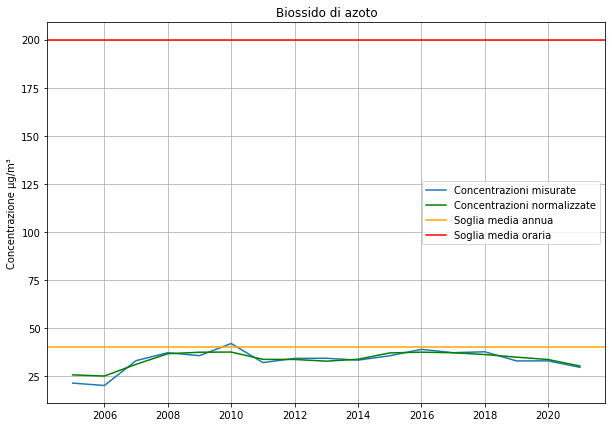
\includegraphics[width=0.75\textwidth]{no2_medie_annuali}
\caption{Confronto tra le medie mensili delle serie storiche rilevate dai sensori e quelle delle serie normalizzate}
\label{fig:no2_medie_annuali}
\end{figure}

\begin{figure}[h]
\centering
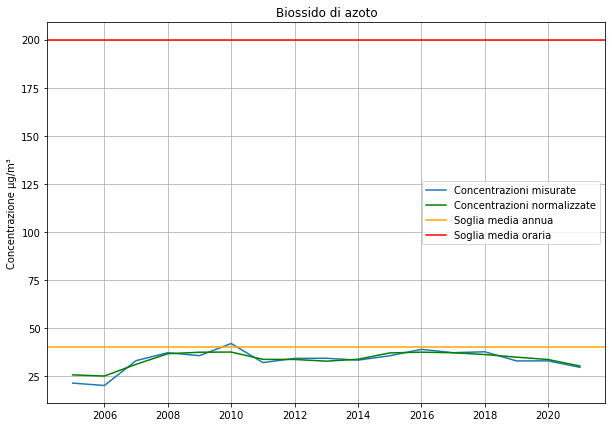
\includegraphics[width=0.75\textwidth]{no2_medie_annuali}
\caption{Confronto tra le medie annuali delle serie storiche rilevate dai sensori e quelle delle serie normalizzate}
\label{fig:no2_medie_annuali}
\end{figure}

Anche per il biossido considerato separatamente le serie ottenute presentano un andamento abbastanza costante e anche in questo caso sembra che dal 2016 le concentrazioni siano leggermente in calo, anche se già in passato (2010-2013) si erano verificati andamenti simili, salvo poi essere tornate ad aumentare negli anni successivi.
Sicuramente è importante notare che le medie annuali delle serie normalizzate rimangano sempre sotto alla soglia imposta dalla normativa vigente, a segno che comunque la situazione per quanto riguarda questo inquinante non sia gravemente critica. Questo non significa che non sia importante monitorarla ed occuparsene, visto che comunque in casi di particolari condizioni atmosferiche può capitare che si abbiano delle situazioni leggermente problematiche, ma di certo le concentrazioni di questo inquinante non possono essere considerate un pericolo attualmente.

C'è inoltre da dire che nel corso dei prossimi anni questo inquinante potrebbe ulteriormente calare, poichè l'innovazione tecnologica, soprattutto per quanto riguarda il mondo delle auto e il rinnovo della flotta circolante porteranno ad avere ulteriori abbassamenti delle emissioni. Chiaramente ci si può aspettare di vedere un processo simile anche per quanto riguarda le combustioni industriali e civili, che sono gli altri due settori importanti per quanto riguarda questo inquinante e che potrebbero dare un buon contributo nel contenimento delle concentrazioni.

\section{PM10 e PM2.5}
Le polveri sottili sono sicuramente l'inquinante più discusso degli ultimi anni essendo quello le cui concentrazioni fanno registrare il maggior numero di superamenti della soglia imposta per legge e del quale è noto l'elevato impatto ambientale e sulla salute degli esseri viventi. Questo fa sì che si accendano spesso dibattiti sulla qualità reale dell'aria che respiriamo e su quali misure siano necessarie per riuscire a mantenere le concentrazioni sotto al valore limite oltre il quale il WHO ha riconosciuto la possibilità di avere danni alla salute.\cite{world2016air} Prima di andare ad analizzare i dati è però bene aver chiaro il contesto in cui si svolgeranno queste analisi. Il particolato infatti è un inquinante molto legato alla stagionalità, sia perchè le condizioni meteorologiche invernali sono più favorevoli all'accumulo rispetto a quelle estive che per le maggior emissioni antropiche tipiche della stagione, causate, ad esempio, dall'uso dei riscaldamenti. Va inoltre ricordato che la Lombardia, come tutto il bacino padano in generale, si trova in una posizione geografica sfavorevole, che porta alla maggior formazione di accumuli, soprattutto durante il periodo invernale.

Il particolato classicamente viene diviso in due categorie: PM10 e PM2.5, a seconda del diametro aerodinamico delle particelle esaminate. Quindi particelle con questo diametro, che non si riferisce alla dimensione della particella ma alla sue caratteristiche aerodinamiche, al di sotto dei 10$\mu$m sono classificate come PM10 e il discorso analogo vale anche per il PM2.5. Essendo appunto particelle molto piccole risultano quindi pericolose per la salute poichè riescono a penetrare più a fondo nell'apparato respiratorio, arrivando quindi ad arrecare danni maggiori. La pericolosità del particolato non deriva solamente dalla sua composizione, che è molto varia per le diverse origini che può avere, ma anche dal fatto che fa da veicolante per altri inquinanti più pericolosi, che si legano in atmosfera e vengono poi trasportate all'interno del corpo dalla particella. Questo inquinante ha appunto origini molto varie, sia di tipo primario da attività come le industrie, i riscaldamenti, il traffico e le combustioni in generale, ma anche di tipo secondario, poichè in atmosfera può formarsi a seguito di trasformazioni chimico-fisiche di altre sostanze.

Secondo INEMAR 2017 la categoria maggiormente responsabile per le emissioni di questi inquinanti sono le combustioni non industriali, quindi, ad esempio, i riscaldamenti domestici, specialmente quelli a biomasse. Il contributo di questa categoria si aggira intorno al 45\% per quanto riguarda il PM10 ed al 50\% per il PM2.5. Al secondo posto troviamo il traffico, con un contributo che arriva al 25\% per quanto riguarda la frazione più grossa del particolato e del 20\% per la più piccola. Per quanto riguarda i combustibili, il legno è di gran lunga il maggior responsabile delle emissioni di particolato, con oltre il 50\% del totale. Il diesel si ferma invece a solo circa il 10\%.

Il PM10 è regolato dall'inizio degli anni 90, con i decreti già citati per gli ossidi di azoto che hanno introdotto limiti e nuove regolamentazioni per le emissioni degli impianti.Per quanto riguarda il settore del traffico l'introduzione più importante è stata quella del filtro antiparticolato nelle marmitte, che permette di ridurre drasticamente le emissioni, insieme chiaramente alle progressive limitazioni imposte tramite le categorie EuroX. Quando si parla di traffico e polveri sottili è importante ricordare che i motori a benzina non generano questo inquinante ed infatti le loro emissioni non sono normate nemmeno dalle sopracitate categorie internazionali.

Per quanto riguarda il PM10 il D.Lgs 155/2010 impone i limiti di 50$\mu g/m^3$ come media giornaliera, che non deve essere superata in più di 35 occasioni all'anno, e 40$\mu g/m^3$ per la media annuale.

Nei modelli ottenuti per trattare questo inquinante la variabile più importante è risultata, non sorprendentemente vista la sua azione dispersiva, la velocità del vento con un valore di 0.20. Al secondo posto troviamo la temperatura (0.18) ed al terzo il giorno dell'anno (0.15), che sono collegate al classico andamento stagionale che fanno registrare le concentrazioni di questo inquinante. Anche al numero di giorni dalle ultime precipitazioni registrate è stata data un'importanza discreta (0.1) anche se nemmeno in questo dovrebbe sorprenderci visto che è noto come la pioggia abbatta le concentrazioni portando al suolo parte del particolato presente in atmosfera. La sua assenza prolungata, soprattutto in periodi come quello invernale dove la dispersione naturale è resa più difficile dalle condizioni climatiche, causa sempre innalzamenti delle concentrazioni registrate che sul territorio lombardo sono frequente causa dei superamenti ai limiti imposti dalla normativa vigente. Grazie all'importanza ottenuta possiamo quindi capire che i modelli costruiti sono stati capaci di anche rilevare questo tipo di dinamica e perciò riescono anche ad eliminarne gli effetti più efficacemente.

\begin{figure}[h]
\centering
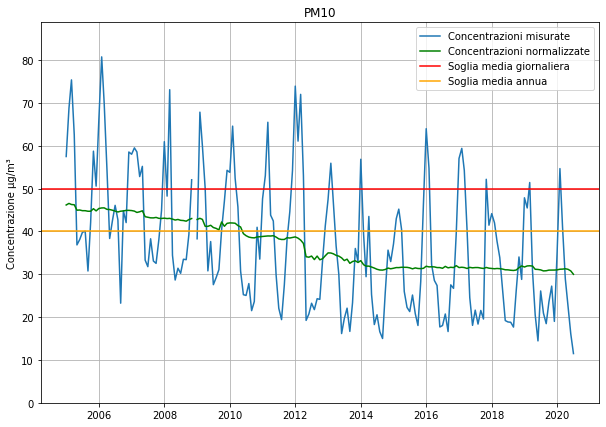
\includegraphics[width=0.75\textwidth]{pm10_medie_mensili}
\caption{Confronto tra le medie mensili delle serie storiche rilevate dai sensori e quelle delle serie normalizzate}
\label{fig:pm10_medie_mensili}
\end{figure}

\begin{figure}[h]
\centering
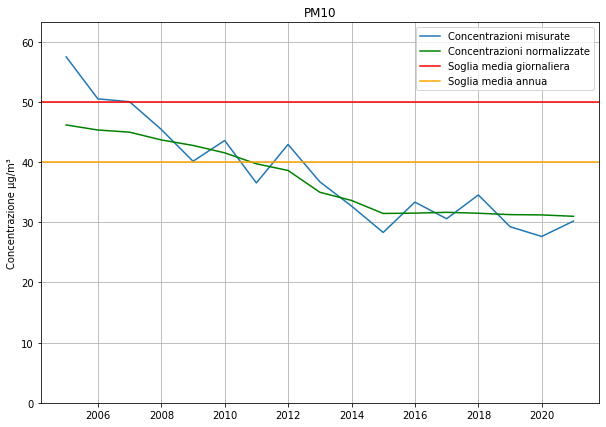
\includegraphics[width=0.75\textwidth]{pm10_medie_annuali}
\caption{Confronto tra le medie annuali delle serie storiche rilevate dai sensori e quelle delle serie normalizzate}
\label{fig:pm10_medie_annuali}
\end{figure}

Nei grafici ottenuti è evidente la presenza di un trend in costante calo, diversamente da quanto visto per gli ossidi di azoto, anche se negli ultimi anni sembra aver rallentato molto ed i valori sono rimasti piuttosto costanti.
Importante notare come successivamente al 2012 le concentrazioni normalizzate siano rimaste sempre sotto al limite per la media annuale di 40$\mu g/m^3$, sia per quanto riguarda le medie annuali che per quelle mensili.
Ancora una volta vediamo come le serie normalizzate ottenute mantengano un andamento medio rispetto ai dati grezzi, a conferma nuovamente della validità dei risultati ottenuti tramite questa tecnica.
Guardando i grafici nelle figure\ref{fig:pm10_medie_mensili}\ref{fig:pm10_medie_annuali} sembrerebbe quasi che nel corso degli ultimi anni si possa aver raggiunto una sorta di limite, dovuto dalla quantità di attività antropiche (e in parte probabilmente anche da un fondo naturale) presenti nella nostra regione, oltre il quale sarà più complicato scendere ulteriormente senza radicali cambiamenti che riescano ad eliminare alcune fonti emissive. Dalla serie ottenuta si capisce che mediamente la situazione per quanto riguarda questo inquinante non è critica, poichè con condizioni climatiche medie le concentrazioni sarebbero sempre sotto ai limiti legislativi. A causare i superamenti, che avvengono quasi tutti nei mesi invernali, sono invece le condizioni climatiche sfavorevoli di quei mesi che, unitamente all'uso dei riscaldamenti domestici ed in generale ad un maggior consumo energetico, portano il particolato ad accumularsi in atmosfera senza riuscire a disperderlo.

Allo stesso modo abbiamo trattato il PM2.5, per il quale ricordiamo che il limite di legge è fissato a 25$\mu g/m^3$ sulla media annua, introdotto per la prima volta a partire dal D.Lgs 155/2010.

\begin{figure}[h]
\centering
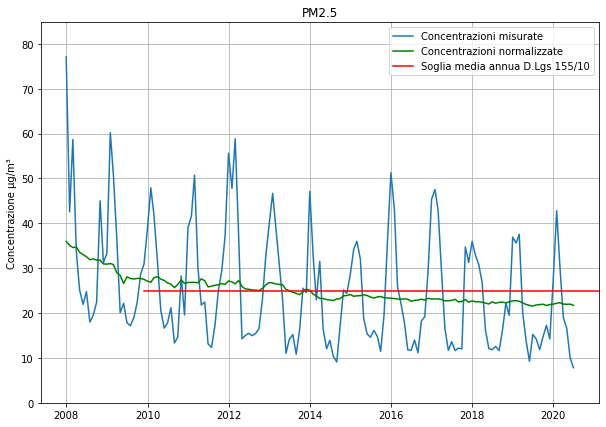
\includegraphics[width=0.75\textwidth]{pm25_medie_mensili}
\caption{Confronto tra le medie mensili delle serie storiche rilevate dai sensori e quelle delle serie normalizzate}
\label{fig:pm25_medie_mensili}
\end{figure}

\begin{figure}[h]
\centering
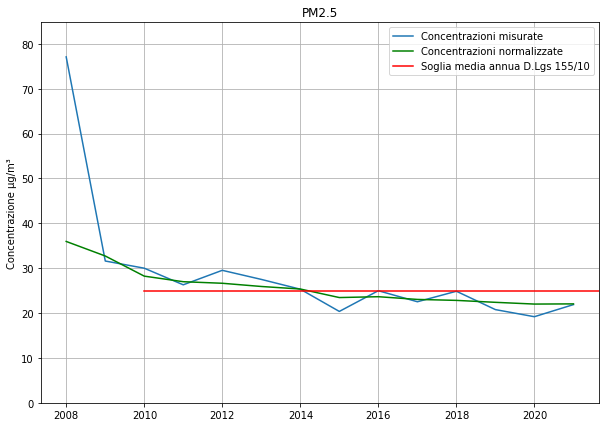
\includegraphics[width=0.75\textwidth]{pm25_medie_annuali}
\caption{Confronto tra le medie annuali delle serie storiche rilevate dai sensori e quelle delle serie normalizzate}
\label{fig:pm25_medie_annuali}
\end{figure}

Anche per questo inquinante viene evidenziato un trend negativo leggermente minore di quanto riscontrato col PM10 e che negli ultimi anni presenta la stessa tendenza al rallentamento, rinforzando i sospetti di aver raggiunto un limite che per essere passato necessità di forti innovazioni che riescano ad eliminare le emissioni già alla fonte.
Abbiamo notato come dal 2015 le concentrazioni normalizzate siano riuscite anche a scendere sotto al limite di legge imposto e come, anche in questo caso, siano fortemente influenzate dalle condizioni sfavorevoli che poi portano spesso ad avere episodi problematici.

\section{CO}
Il monossido di carbonio è un inquinante molto pericoloso per la salute, in quanto è nota la sua migliore capacità di legarsi all'emoglobina rispetto all'ossigeno, causando notevoli danni per l'uomo\cite{kao2005carbon}.
È un inquinante che viene prodotto da combustioni in difetto di ossigeno ed ha origine prevalentemente primaria, essendo emesso direttamente da tutti i processi di combustione incompleta dei composti carboniosi (gas naturali, propano, carburanti, benzine, carbone, legna, ecc..).

Secondo quanto riportato da INEMAR 2017 i due settori maggiormente responsabili delle emissioni di questo inquinante sono il traffico ed i riscaldamenti domestici e le combustioni non industriali, con un contributo pari rispettivamente al 38\% e 27\% del totale delle emissioni annue. Le emissioni collegate al settore dei trasporti hanno fatto registrare forti cali a partire dagli anni 90, con una riduzione vicina addirittura al 90\% favorita da innovazioni quali le marmitte catalitiche e in generale il progresso tecnologico che, per esempio, ha permesso di passare dai 12,66gCO/km emessi dai motori a benzina classificati come Euro 0 (quelli antecedenti all'istituzione delle normative europee) a 1gCO/km che viene imposto come limite per la categoria Euro 6.
Per quanto riguarda invece il settore dei riscaldamenti domestici nel corso degli ultimi anni le emissioni hanno seguito un trend sempre crescente, causato soprattutto dall'uso della legna come combustibile, che però porta effetti riscontrabili solo localmente dove è più utilizzata (e solitamente le aree cittadine non sono questo tipo di zone, anche perchè il loro uso è fortemente limitato e regolamentato dalla normativa attuale).

Il limite di legge alle concentrazioni di questa sostanza in atmosfera è fissato a 10 $\mu g/m^3$ a partire dal 2005, anche se ormai sono più di vent'anni che non vengono registrati valori maggiori. Il monossido, quindi, ormai non rappresenta più un problema e le sue concentrazioni in atmosfera sono molto vicine al fondo naturale\cite{arpa2018rapporto} e spesso si arriva anche ai limiti della rilevabilità da parte dei sensori.
Pur non essendo più un problema abbiamo ritenuto che potesse comunque valer la pena di analizzare la situazione anche per quanto riguarda questo inquinante, ripetendo quanto fatto in precedenza per gli altri.

Nei modelli la temperatura è risultata essere la variabile con l'importanza maggiore (0.26), in quanto funziona da proxy per la stagionalità e quindi anche per l'uso dei riscaldamenti domestici. Al secondo posto troviamo il giorno dell'anno (0.18) ed al terzo la data, che può essere un indizio di come l'andamento della serie reale possa essere caratterizzato da variazioni non dovute ai fattori meteorologici considerati come potrebbero essere le oscillazioni nel fondo naturale.

\begin{figure}[h]
\centering
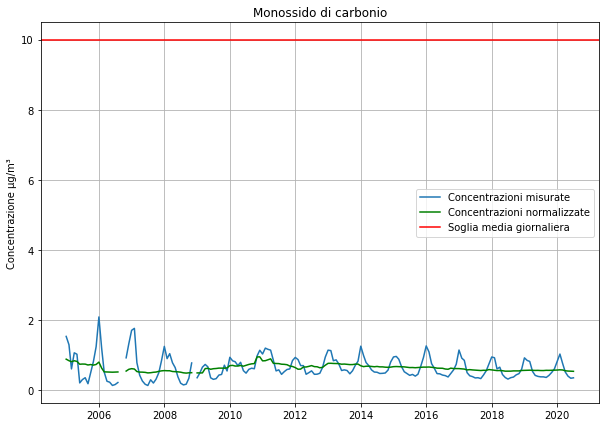
\includegraphics[width=0.75\textwidth]{co_medie_mensili}
\caption{Confronto tra le medie mensili delle serie storiche rilevate dai sensori e quelle delle serie normalizzate}
\label{fig:co_medie_mensili}
\end{figure}

\begin{figure}[h]
\centering
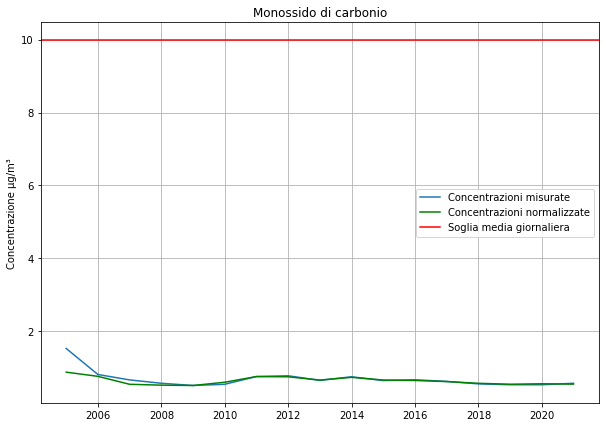
\includegraphics[width=0.75\textwidth]{co_medie_annuali}
\caption{Confronto tra le medie annuali delle serie storiche rilevate dai sensori e quelle delle serie normalizzate}
\label{fig:co_medie_annuali}
\end{figure}

Dal 2006 ad oggi le concentrazioni di monossido di carbonio sono rimaste piuttosto stabili, mostrando un andamento abbastanza costante, con un leggero aumento tra il 2010 e il 2014, seguito poi però da una fase di leggero calo. Questo andamento, che risulta praticamente costante e caratterizzato da variazioni piuttosto casuali, può sicuramente farci pensare di essere vicini alla misura del fondo naturale per questo inquinante, che ormai da anni non rappresenta più un problema.
Va infatti notato come nel periodo preso in esame i valori siano sempre rimasti sotto al 1 $\mu g/m^3$, ben più bassi del limite imposto dalla legge. Inoltre le medie delle serie normalizzate seguono abbastanza bene quelle delle concentrazioni reali, facendoci quindi pensare che le fluttuazioni possano essere più oscillazioni nel valore del fondo naturale che cambiamenti dovuti ad attività umane o altri fattori come quelli considerati dal nostro modello.

\section{Ozono}
L'ozono troposferico è un inquinante di origine secondaria, che si forma in atmosfera quando, favoriti da alte temperature e forte irraggiamento, ossidi di azoto e composti organici volatili subiscono trasformazioni chimico-fisiche che portano alla sua formazione. Per questo motivo l'ozono è considerato smog fotochimico ed il periodo critico per le sue concentrazioni, a differenza degli altri inquinanti, è quindi l'estate.\cite{seinfeld1988ozone}
I precursori dell'ozono arrivano generalmente da combustioni civili ed industriali e da processi che usano o producono sostanze chimiche volatili, ma avendo una formazione più complessa è chiaramente più difficile capire quali siano le sue origini e quindi dove intervenire per controllarne efficacemente le concentrazioni.

L'ozono è noto per la sua pericolosità per l'apparato respiratorio, al quale può causare problemi temporanei anche a seguito di un'esposizione a basse concentrazioni; chiaramente se l'esposizione avviene in modo ripetuto o prolungato il rischio di avere dei danni permanenti aumenta. In generale comunque, soprattutto ad alte concentrazioni, l'ozono diventa pericoloso sia per gli esseri umani che per la vegetazione, sulla quale può avere effetti negativi.

La normativa attuale fissa a 120 $\mu g/m^3$ il valore obbiettivo per la media mobile calcolata su 8 ore, con un massimo di 25 superamenti annui calcolati sulla media di 3 anni. Attualmente questo limite viene rispettato a fatica (nel 2018 nella provincia di Milano tutte le stazioni l'hanno abbondantemente superato), ma ciò comunque non costituisce una criticità per la regione, in quanto questi superamenti sono tutti collegati al classico andamento stagionale.\cite{arpa2018rapporto}

Nei modelli ottenuti per la trattazione dell'ozono le due variabili nettamente più importanti si sono rivelate essere la radiazione (0.33) e la temperatura (0.32), dimostrando quindi che sono stati capaci di interpretare perfettamente le dinamiche che portano alla maggior formazione di questo inquinante.

\begin{figure}[h]
\centering
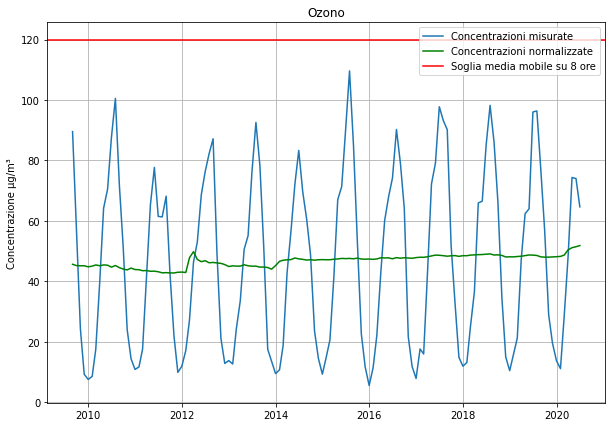
\includegraphics[width=0.75\textwidth]{o3_medie_mensili}
\caption{Confronto tra le medie mensili delle serie storiche rilevate dai sensori e quelle delle serie normalizzate}
\label{fig:o3_medie_mensili}
\end{figure}

\begin{figure}[h]
\centering
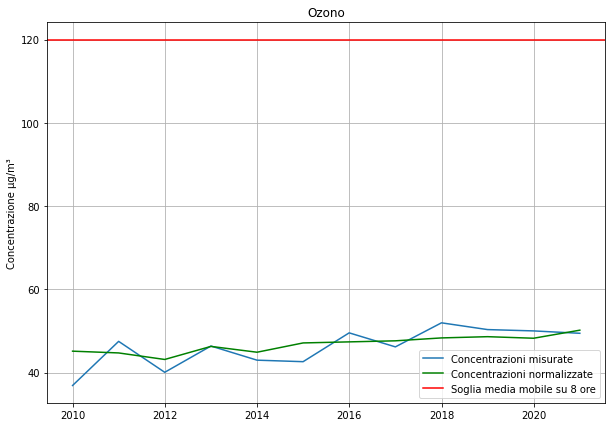
\includegraphics[width=0.75\textwidth]{o3_medie_annuali}
\caption{Confronto tra le medie annuali delle serie storiche rilevate dai sensori e quelle delle serie normalizzate}
\label{fig:o3_medie_annuali}
\end{figure}

L'andamento delle concentrazioni a partire dal 2013 è leggermente in aumento con una crescita del 10\%. L'ozono, per la sua origine complessa, è molto difficile da tracciare e quindi diventa complicato anche intervenire per contenerne le concentrazioni in modo efficace. Attualmente la situazione in Lombardia non risulta problematica, ma il trend in aumento richiede di porre attenzione alla situazione di questo inquinante.

Un aspetto da notare è che l'ozono, tra tutti gli inquinanti, è quello che la nostra tecnica riesce a trattare con la maggiore precisione ed infatti i modelli ottenuti usati per ricavare le serie normalizzate sono quelli che in fase di costruzione hanno mostrato le performance migliori. Questo probabilmente è collegato alla forte relazione che questo inquinante ha con la temperatura e, soprattutto, la radiazione solare, che i nostri modelli hanno ben individuato (come si è visto con l'importanza delle variabili) e che quindi gli permetteva di essere più precisi nell'attività predittoria.

\section{Ammoniaca}
L'ammoniaca è un inquinante prodotto da processi degradativi di sostanza organica, le cui principali sorgenti sono infatti attività agricole e, in misura minore, il traporto su strada e la combustione di legna e combustibili fossili. È un gas molto solubile in acqua e questo lo rende pericoloso poichè può essere causa dell'acidificazione dei suoli. Inoltre negli ultimi l'interesse per l'ammoniaca è sempre crescente a causa della sua partecipazione nella formazione di particolato secondario quando presente in atmosfera.

Secondo INEMAR2017 in Lombardia il 96\% delle emissioni di questa sostanza sono collegabili al settore dell'agricoltura, che infatti è il principale responsabile per quanto riguarda questo inquinante. Il traffico, invece, arriva a dare un contributo pari solamente al 1\% del totale annuo.

La normativa attuale non impone limiti per le concentrazioni registrate, anche se una serie di direttive europee per lo sviluppo rurale ha mirato, nel corso degli anni, a favorire la diffusione di buone pratiche per contenerne le emissioni, come ad esempio il divieto dello spargimento di liquami. 

Nei modelli ottenuti la variabile più importante è risultata essere la data (0.35), seguita dal giorno dell'anno (0.14) e dalla temperatura (0.11). Anche in questo caso, in cui alla data viene data un'importanza molto alta, potremmo trovarci nella stessa situazione che già parizalmente si era vista per il monossido di carbonio. L'andamento di questo inquiante, infatti, probabilmente è regolato da fenomeni diversi di quelli considerati dalle nostre variabili e quindi la data stessa risulta essere l'informazione migliore per fare previsioni sulle concentrazioni di ammoniaca in tale data.

%inserisci grafici
\begin{figure}[h]
\centering
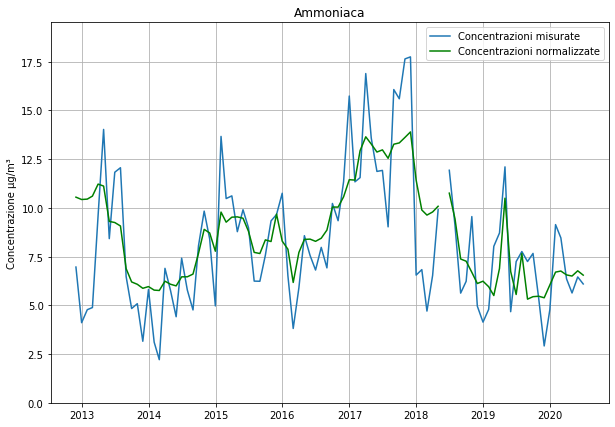
\includegraphics[width=0.75\textwidth]{ammoniaca_medie_mensili}
\caption{Confronto tra le medie mensili delle serie storiche rilevate dai sensori e quelle delle serie normalizzate}
\label{fig:ammoniaca_medie_mensili}
\end{figure}

\begin{figure}[h]
\centering
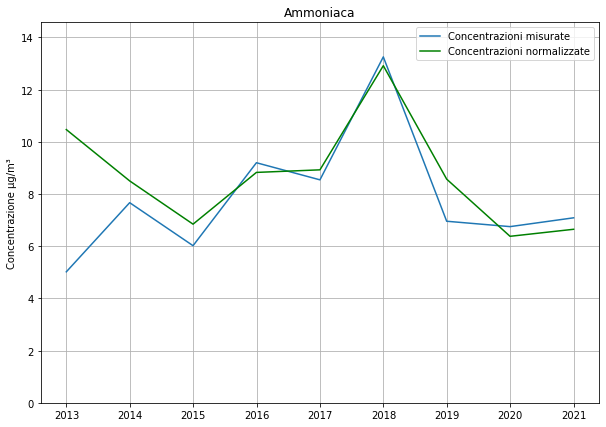
\includegraphics[width=0.75\textwidth]{ammoniaca_medie_annuali}
\caption{Confronto tra le medie annuali delle serie storiche rilevate dai sensori e quelle delle serie normalizzate}
\label{fig:ammoniaca_medie_annuali}
\end{figure}

Come si vede nei grafici delle figure\ref{fig:ammoniaca_medie_mensili}\ref{fig:ammoniaca_medie_annuali} l'andamento delle serie normalizzate ottenute rispecchia abbastanza fedelmente quello delle concentrazioni realmente misurate. Questa è quindi un'ulteriore dimostrazione di come l'influenza della meteorologia su questo inquinante sia praticamente nulla, visto che dopo averne teoricamente eliminato gli effetti si ottiene ancora una serie molto simile.

\section{Benzene}
Il benzene viene sintetizzato dal petrolio e viene usato per produrre materie plastiche e soprattutto come sostanza antidetonante nella benzina. Il benzene, infatti, ad inizio anni 90 ha sostituito il piombo come additivo presente in essa, permettendo il passaggio da quella rossa a quella verde.
Quello presente in atmosfera deriva da processi di combustione incompleta di combustibili fossili, quindi da attività come traffico (soprattutto dai veicoli a benzina) e processi di combustione industriale.

La sua pericolosità per la salute umana varia molto a seconda della concentrazione e della durata dell'esposizione, ma anche alle basse quantità a cui viene misurato in atmosfera può comunque essere pericoloso: lo IARC (agenzia internazionale per la ricerca sul cancro) l'ha infatti inserito tra le sostanze per le quali esiste una sufficiente evidenza di cancerogenicità per l'uomo.\cite{iarc2018benzene}

Il D.Lgs 155/2010 stabilisce per questo inquinante un valore limite di 5$\mu g/m^3$ per la media oraria, che viene ormai ampiamente rispettato in tutta la regione. Questo inquinante, che in passato era più problematico, è stato drasticamente ridotto grazie a diverse misure come la riduzione del suo tenore nelle benzine e l'adozione del ciclo chiuso e dei catalizzatori nelle marmitte. 

Nei modelli ottenuti l'importanza delle variabili si è rivelata essere abbastanza in linea con quanto visto per gli altri inquinanti, con temperatura, giorno dell'anno e data che risultano essere le più importanti.

\begin{figure}[h]
\centering
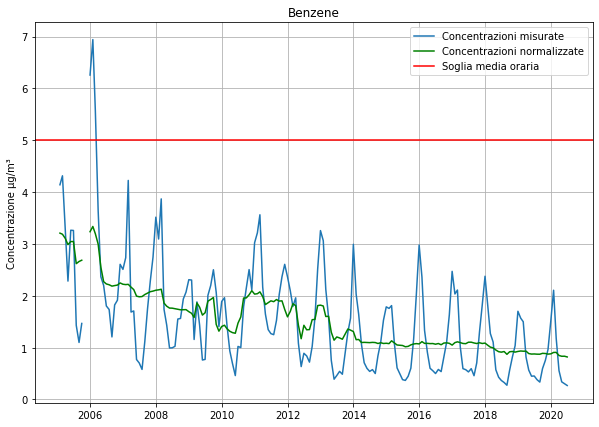
\includegraphics[width=0.75\textwidth]{benzene_medie_mensili}
\caption{Confronto tra le medie mensili delle serie storiche rilevate dai sensori e quelle delle serie normalizzate}
\label{fig:benzene_medie_mensili}
\end{figure}

\begin{figure}[h]
\centering
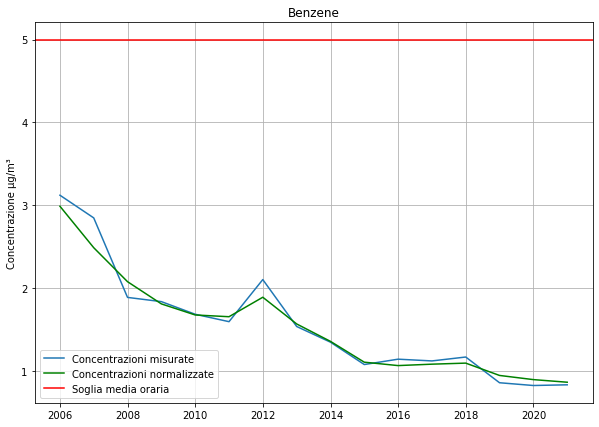
\includegraphics[width=0.75\textwidth]{benzene_medie_annuali}
\caption{Confronto tra le medie annuali delle serie storiche rilevate dai sensori e quelle delle serie normalizzate}
\label{fig:benzene_medie_annuali}
\end{figure}

Nei grafici in figure\ref{fig:benzene_medie_mensili}\ref{fig:benzene_medie_annuali} sono riportati gli andamenti delle serie reali e normalizzate di questo inquinante. Si nota chiaramente un costante trend in calo, dovuto alle misure sopracitate, che hanno permesso, nonostante l'aumento dei volumi di traffico, di abbattere le concentrazioni ad un livello che ormai non risulta più pericoloso per la salute umana.

\section{SO2}
Sebbene una volta fosse sicuramente uno degli inquinanti a destare più proccupazioni, così come è stato uno dei primi ad essere monitorato e limitato per legge, è già ormai diversi anni che le concentrazioni di biossido di zolfo sono ampiamente sotto al limite legislativo per questo inquinante (350 $\mu g/m^3$ media oraria), visto che a partire dagli anni 90 sono state introdotte una serie di normative atte a limitarne le emissioni. Le più importanti sono sicuramente quelle riguardanti gli usi di gasolio e nafta come forme di riscaldamento, che ormai sono stati completamente sostituiti dal metano, e quelle che nel corso degli anni hanno progressivamente abbassato il limite di zolfo che può essere contenuto nei carburanti (da 0.8\% nel 1980 a 0.2\% nel 1995 e infine a 0.1\% nel 2008).

Sebbene non vi siano più preoccupazioni per quanto riguarda le concentrazioni di questa sostanza in atmosfera abbiamo ritenuto che fosse utile verificare anche con essa i risultati ottenuti tramite la nostra tecnica. 

La data è risultata di gran lunga la variabile più importante (0.41), con giorno dell'anno (0.14) e temperatura (0.11) che sono le sole due variabili a cui veniva attribuita un minimo di importanza. Trovare la data come variabile più importante per un inquinante che ormai è arrivato al fondo naturale ci conferma esattamente come le fluttuazioni presenti nelle sue serie siano dovute a fattori esterni a quelli considerati nei nostri modelli.

\begin{figure}[h]
\centering
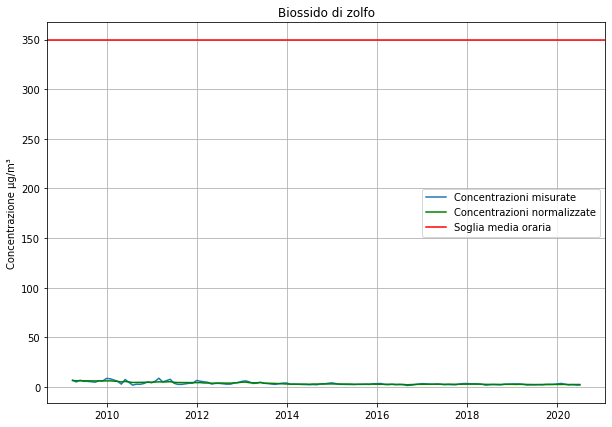
\includegraphics[width=0.75\textwidth]{so2_medie_mensili}
\caption{Confronto tra le medie mensili delle serie storiche rilevate dai sensori e quelle delle serie normalizzate}
\label{fig:so2_medie_mensili}
\end{figure}

\begin{figure}[h]
\centering
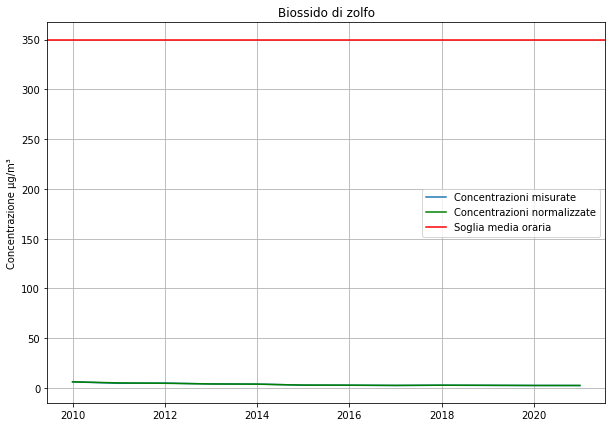
\includegraphics[width=0.75\textwidth]{so2_medie_annuali}
\caption{Confronto tra le medie annuali delle serie storiche rilevate dai sensori e quelle delle serie normalizzate}
\label{fig:so2_medie_annuali}
\end{figure}

Come si può vedere nei grafici\ref{fig_so2_medie_mensili}\ref{so2_medie_annuali} le concentrazioni di SO2 registrate sono ormai a livelli bassissimi, tanto da non destare più preoccupazioni. Come già ampiamente riconosciuto da diversi studi in materia questo inquinante potrebbe essere arrivato al fondo naturale e non c'è motivo di preoccupazione per quanto riguarda la sua situazione attuale.

\chapter{Effetti del traffico sui principali inquinanti atmosferici}
Avere a disposizione una tecnica che ci permette di eliminare l'influenza delle condizioni meteorologiche e della variabilità stagionale dalle concentrazioni degli inquinanti atmosferici ci permette di poter fare delle analisi più precise sull'efficacia di misure prese per contrastare l'inquinamento. L'andamento delle serie normalizzate, infatti, deve per forza essere causato da fattori non considerati nella loro generazione. Sicuramente i due più importanti sono: l'eventuale trend rilevato per le concentrazioni, che noi ovviamente non andiamo ad eliminare poichè è quello che ci interessa per monitorarne l'andamento, ed altri fattori che possono avere un'influenza e che non sono stati considerati, quindi ad esempio particolari situazioni in cui le emissioni antropiche sono state ridotte (COVID) o nuove normative messe in campo.

Quando si parla di inquinamento atmosferico uno degli aspetti su cui sicuramente il dibattito è più acceso e che attira più interesse è l'influenza del traffico veicolare sulla qualità dell'aria. Spesso infatti si sente additare il traffico come il principale responsabile delle concentrazioni degli inquinanti più preoccupanti (e, salvo gli ossidi di azoto, questa cosa non è vera) e sempre maggiori nel corso degli anni sono stati i provvedimenti presi nelle grandi città atti a ridurne i volumi, in nome di una migliore qualità dell'aria. Questi provvedimenti sono stati sempre molto contestati e dibattuti, poichè molti ritengono che il traffico non sia la causa principale dell'inquinamento e che la soluzione non sia bloccarlo ma studiare alternative per renderlo più sostenibile ed efficiente, poichè gli spostamenti in automobile sono comunque una necessità per molte persone.

Il nostro obbiettivo è stato quello di provare ad usare la nostra tecnica per verificare quali siano stati i risultati ottenuti in seguito all'applicazione di alcuni provvedimenti sul traffico presi nella città di Milano nel corso degli ultimi anni, in modo da mostrare come l'applicazione di tecniche per normalizzare i dati dell'inquinamento rispetto alla meteorologia permetta uno studio migliore dell'efficacia delle misure prese nell'abbattimento delle concentrazioni. Purtroppo la mancanza di dati relativi a velocità e direzione del vento, due misure (specialmente la prima) a cui di solito viene assegnata una discreta importanza dai nostri modelli, ci costringe a limitare le nostre analisi al periodo successivo al 2012, ovvero solo successivamente all'introduzione di Area C. Sarebbe stato interessante, ma putroppo non è stato possibile, avere a disposizione anche dati degli anni precedenti, in modo da poter fare un confronto più esteso che coinvolgesse anche il periodo precedente all'entrata in vigore del provvedimento.
Per verificare eventuali effetti derivanti dall'introduzione di questi provvedimenti siamo andati a confrontare l'andamento della serie normalizzata ottenuta per la stazione di Milano Via Senato, coinvolta appunto dal provvedimento Area C, con quelli delle serie di altre due stazioni: quella di Pioltello Limito, situata nell'hinterland milanese, e quella di Bormio, che si trova in un ambiente molto diverso da quello cittadino. La prima è stata scelta poichè, essendo comunque vicina alla città, la qualità dell'aria e le condizioni che la determinano dovrebbero essere abbastanza simili. Non essendo stata colpita da nessun provvedimento, inoltre, ci permette di avere una base di confronto per verificare se appunto l'applicazione di misure come Area C possa effettivamente aver portato a qualche risultato. La stazione di Bormio invece presenta caratteristiche completamente differenti, ma è comunque utile provare a verificare eventuali analogie o discrepanze tra le serie, anche per vedere quali siano le differenze tra due località così diverse.

\section{$NO_x$ e $NO_2$}
\subsection{$NO_x$}
Quando si parla di traffico e si vuole analizzare il suo impatto sulla qualità dell'aria gli inquinanti di maggiore interesse sono sicuramente gli ossidi di azoto, di cui questa categoria risulta responsabile per il 50\% delle emissioni secondo quanto riportato da INEMAR 2017.\cite{inemar2017}

Quando si parla degli ossidi di azoto relativamente al traffico l'attenzione viene posta maggiormente sul diesel, che è il maggior responsabile delle emissioni di questo inquinante. Nel corso degli ultimi anni il numero dei veicoli con motorizzazione diesel circolanti in Italia è andato sempre ad aumentare, tanto che IIR2020\cite{iir2020} stima un consumo quasi triplo di carburante per quanto riguarda veicoli diesel rispetto a quelli a benzina. Questo aumento di veicoli circolanti avrebbe dovuto aver l'effetto di innalzare le concentrazioni di ossidi di azoto misurate, ma è stato contrastato dall'innovazione tecnologica che è riuscita sempre di più a ridurre le emissioni prodotte (basti pensare alle categorie EuroX), introducendo importanti invenzioni come ad esempio la marmitta catalitica.

In precedenza, analizzando  l'andamento della media tra le serie dei capoluoghi di provincia lombardi, avevamo ottenuto un andamento abbastanza costante nel corso degli ultimi 15 anni, con un leggero trend calante negli anni più recenti. Sembra quindi che anche per la Lombardia l'aumento dei veicoli circolanti motorizzati a diesel sia stato contrastato dal progresso tecnologico, che ha permesso di mantenere le concentrazioni sotto controllo.

Abbiamo quindi creato tre modelli per questo inquinante, uno per ogni località scelta per il nostro esperimento, e provato a verificare come negli anni si siano evolute le diverse situazioni.

Innanzitutto abbiamo notato come per tutte e tre le località la velocità del vento sia risultata una variabile a cui è sempre stata assegnata una buona importanza (0.21 a Milano, 0.28 a Limito e 0.34 a Bormio). Per quest'ultima stazione, addirittura, l'importanza risulta di gran lunga più alta rispetto a tutte le altre variabili.  Pensando alle sue caratteristiche geografiche la cosa però non dovrebbe sorprenderci più di tanto, poichè è evidente come in una valle montana l'azione del vento possa avere una funzione dispersiva ancora più importante che in altre località.
L'altra variabile che in tutti e tre i casi è stata riconosciuta come buon predittore risulta essere la temperatura, che può essere utile per verificare sia l'andamento stagionale che possibili eventi meteorologici particolari che possono portare ad un aumento delle emissioni antropiche (ad esempio periodi particolarmente freddi in cui vengono maggiormente usati riscaldamenti e automezzi rispetto a quando si registrano temperature più miti).  

\begin{figure}[h]
\centering
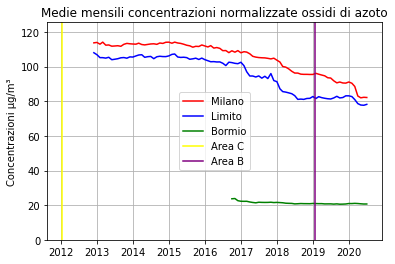
\includegraphics[width=0.75\textwidth]{nox_traffico}
\caption{Confronto degli andamenti delle serie normalizzate calcolate per le stazioni di Milano via Senato, Limito di Pioltello e Bormio}
\label{fig:nox_traffico}
\end{figure}

Dal grafico\ref{fig:nox_traffico} si nota innanzitutto come la serie di Bormio abbia davvero dei valori ridotti che ci mostrano come in località di questo tipo l'inquinamento da ossidi di azoto non sia sicuramente un problema.
Un altro aspetto che risalta subito all'occhio è l'andamento pressochè identico delle serie relative a Milano e Limito, che mostrano entrambe come a partire dal 2016/2017 si sia registrato un trend decrescente praticamente compatibile tra le due stazioni. Analizzando solo la serie di Milano avremmo potuto pensare che questo calo potesse essere collegato alla riduzione del traffico causata dai provvedimenti presi, ma osservare lo stesso andamento anche su una stazione diversa e non colpita da tali limitazioni ci indica che la causa deve per forza essere un'altra. Una possibile idea è che l'origine di questo trend sia proprio nell'innovazione tecnologica, i cui risultati stanno finalmente mettendosi in mostra nonostante le sempre maggiori attività umane, portando a registrare un calo generale e non specifico di alcune località. A Bormio, dove sicuramente la densità di attività antropiche inquinanti è nettamente ridotta rispetto alle altre due stazioni, questo calo risulta chiaramente molto minore, sia appunto perchè gli effetti dell'innovazione possono essere meno evidenti a causa della minor applicazione che perchè le concentrazioni sono già molto ridotte e quindi è ancora più difficile far registrare dei cali consistenti.

\subsection{$NO_2$}
Per completezza è stato trattato anche il biossido di azoto, inquinante sempre molto collegato al traffico e attorno al quale c'è molto interesse per i possibili effetti sulla salute umana.

I modelli creati hanno mantenuto le buone performance viste con quelli creati per trattare gli ossidi ed anche l'importanza delle variabili è risultata praticamente invariata, non sorprendentemente vista la relazione tra le due misure.

\begin{figure}[h]
\centering
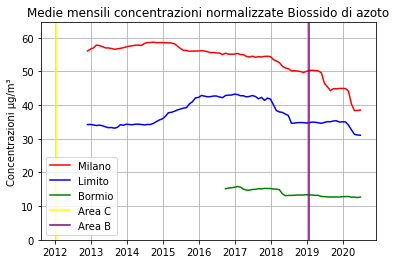
\includegraphics[width=0.75\textwidth]{no2_traffico}
\caption{Confronto degli andamenti delle serie normalizzate calcolate per le stazioni di Milano via Senato, Limito di Pioltello e Bormio}
\label{fig:no2_traffico}
\end{figure}

In questo caso notiamo una sostanziale differenza tra l'andamento delle serie di Milano e Limito. La prima, in modo abbastanza compatibile con quanto già visto per gli ossidi di azoto, mostra un trend decrescente a partire dagli ultimi cinque anni\ref{fig:no2_traffico}. Per la seconda, invece, tra gli anni 2015 e 2018 si è assistito ad un aumento delle concentrazioni, che prima si mantenevano su un livello abbastanza stabile, che sono tornate a riscendere nel corso degli ultimi due anni. È proprio negli stessi anni in cui la serie normalizzata fa registrare questo aumnento che proprio in quella zona è stata inaugurata l'autostrada BreBeMi, che potrebbe aver portato ad un aumento del flusso di traffico e conseguentemente delle concentrazioni registrate. Andrebbe però verificato per quale motivo a seguito del 2018 sembra che le concentrazioni tornino sul livello più o meno costante visto tra il 2012 ed il 2014.
Per quanto riguarda la situazione di Milano sembra che effettivamente la qualità dell'aria sia migliorata nel corso degli anni, potenzialmente anche grazie alla riduzione del traffico causata da Area C prima ed Area B poi, visto che proprio qualche mese dopo l'introduzione di questo provvedimento il nostro modello ha effettivamente rilevato un calo intorno al 10\% nelle concentrazioni di biossido. Se questa è sicuramente una potenziale causa è anche vero che probabilmente a contribuire ai ribassamenti c'è un trend di fondo, dettato da fattori come l'innovazione tecnologica, che infatti sembra parzialmente verificato anche per Pioltello (almeno a seguito del 2018) che per Bormio.

Per quanto riguarda gli ossidi di azoto i nostri modelli sembra che effettivamente mostrino un calo intorno al 10\% a seguito dell'introduzione di Area B. Sarebbbe interessante poter comparare questo calo col numero di veicoli che a causa di questa misura non hanno più circolato, per capire se possa esistere una corrsipondenza tra i due dati. Dall'altra parte, però, questo calo risulta comunque minimo e sicuramente minore di quello dovuto al trend mostrato dalle concentrazioni, che dal 2012 ad oggi hanno mostrato un calo intorno al 33\% sia per gli ossidi che per il biossido considerato singolarmente, e che è sicuramente collegato col progresso tecnologico che ha portato alla riduzione delle emissioni.

\section{CO}
Per quanto riguarda il monossido di carbonio INEMAR 2017 individua trasporto su strada e combustioni non industriali (quindi i riscaldamenti, in particolare quelli alimentati a biomasse) come le due principali fonti emissive, con un percentuale di circa il 60\% del totale.

La situazione per quanto riguarda questo inquinante non risulta essere critica, visto che le concentrazioni registrare sono ormai prossime a valori riconducibili al fondo naturale. Nonostante ciò abbiamo ritenuto fosse comunque utile fare un'analisi di questo tipo, sia per verificare eventuali effetti dei provvedimenti di limitazione al traffico presi, che per provare a cercare eventuali differenze tra le serie delle tre località. In questo caso risulta particolarmente interessante indagare anche su quella di Bormio, poichè è una zona in cui la legna viene ancora molto usata come forma di riscaldamento e quindi si possono indagare su quali siano gli effetti di questi "comportamenti".

La variabile con importanza maggiore nei tre modelli è stata la temperatura (0.20 a Milano, 0.34 a Limito e 0.19 a Bormio), che gli permette proprio di cogliere l'andamento tipicamente stagionale di questo inquinante. Inoltre, essendo derivante in buona parte dai riscaldamenti domestici, è abbastanza evidente come tale misura possa essere utilizzata per stimarne un loro utilizzo e quindi riuscire a fare previsioni più precise e che sappiano fare da proxy anche questo aspetto.
La velocità del vento, chiaramente, ha ottenuto ancora una buona importanza, che ci conferma nuovamente la forte azione dispersiva di questo elemento.
Per quanto riguarda il modello di Bormio abbiamo visto che la radiazione globale sia risultata essere la variabile con importanza maggiore (0.19), al pari della temperatura. Anche per essa e per il collegamento con la presenza di sole (e quindi il possibile uso di riscaldamenti) e la stagionalità è naturale che valga lo stesso discorso fatto per la temperatura.

\begin{figure}[h]
\centering
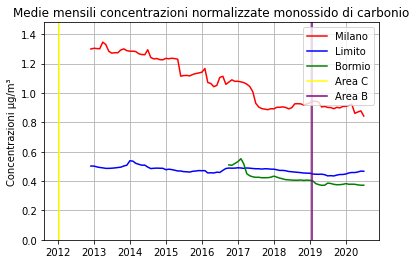
\includegraphics[width=0.75\textwidth]{co_traffico}
\caption{Confronto degli andamenti delle serie normalizzate calcolate per le stazioni di Milano via Senato, Limito di Pioltello e Bormio}
\label{fig:co_traffico}
\end{figure}

Se le stazioni di Limito e Bormio presentavano valori già molto bassi e con un andamento costante, per la stazione di Milano, nel grafico in figura\ref{fig:co_traffico} possiamo vedere che nel corso degli ultimi anni si sia registrato un calo abbastanza importante delle concentrazioni. Attualmente i valori risultano ancora più alti rispetto a quelli delle altre due località, potenzialmente anche a causa della maggior densità abitativa (e quindi un maggiore uso di veicoli e riscaldamenti) della città rispetto alle altre due zone.
L'origine di questo calo potrebbe sicuramente essere in parte collegata i provvedimenti di limitazione del traffico, come potrebbe venire il sospetto guardando il grafico, poichè viene registrato solo per la stazione di Milano e non sulle altre due (a differenza di quanto visto in precedenza dove il calo risultava essere compatibile su tutte le località). Altre possibili ragioni potrebbero essere i provvedimenti di limitazione all'uso di riscaldamenti a biomasse nelle città presi nel corso degli ultimi anni, anche se il loro effetto probabilmente si sarebbe dovuto vedere, anche solo parzialmente, anche sulle serie delle altre località, in particolare quella di Limito che è stata soggetta alle stesse limitazioni.

\section{PM10}
Le polveri sottili sono sempre un inquinante molto discusso e che spesso viene (anche erroneamente) collegato al traffico. Secondo INEMAR 2017\cite{inemar2017} il traffico risulta essere responsabile di meno del 25\% delle emissioni di PM10, mentre il settore principale risultano ancora essere le combustioni non industriali, specialmente per quanto riguarda i riscaldamenti a biomasse. Avendo una composizione molto varia è comunque difficile stabilire in modo preciso l'origine del particolato atmosferico e quindi quali siano le fonti di maggiori emissioni.
Una cosa che però è bene ricordare quando si parla di polveri sottili e traffico è che gli unici responsabili di questo inquinante per questo settore sono i motori a diesel, poichè quelli a benzina non lo producono (ed infatti non viene limitato nemmeno dalle categorie EuroX).

Negli ultimi anni c'è stata molta attenzione riguardo a questo inquinante, specialmente per gli effetti che ha sulla salute umana.
Questo ha quindi portato anche molto interesse nella ricerca di soluzioni efficaci per il loro contenimento, che per quanto riguarda il traffico sono state individuate nell'uso di filtri antiparticolato che riducano le emissioni al tubo di scappamento. 

Anche in queste trattazioni si è riscontrato come la nostra tecnica abbia sempre prestazioni leggermente peggiori quando si vanno a trattare le polveri sottili, probabilmente a causa del fatto che le variabili da noi considerate non siano sufficentemente in grado di spiegare i fenomeni su più larga scala che influenzano le loro concentrazioni.

\begin{figure}[h]
\centering
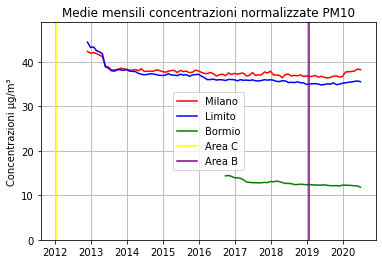
\includegraphics[width=0.75\textwidth]{pm10_traffico}
\caption{Confronto degli andamenti delle serie normalizzate calcolate per le stazioni di Milano via Senato, Limito di Pioltello e Bormio}
\label{fig:pm10_traffico}
\end{figure}

Dal grafico\ref{fig:pm10_traffico} notiamo come l'andamento delle tre serie, sebbena quella di Bormio stia su valori molto minori, sia assolutamente compatibile con grande similitudine tra quella di Milano e quella di Limito e vista la natura del particolato, che viene trasportato anche per grandi distanze, la cosa comunque non ci stupisce. In questo caso si vede come non si possa notare alcuna differenza tra gli andamenti delle serie che ci possa suggerire una reale efficacia dei provvedimenti presi in termini di limitazione del traffico. Anzi, guardando il grafico ottenuto, la serie di Limito (non coinvolto da nessuna misura) risulta calata leggermente di più rispetto a quella di Milano.
Il trend ricavato è calante ma i valori sono sicuramente ancora molto vicini al limite imposto per legge e questa potrebbe essere un'indicazione della necessità di misure di diverso tipo per contrastare questo inquinante, che dovranno necessariamente coinvolgere i settori maggiormente responsabili delle emissioni e non solamente il traffico.

\section{Utilizzo di dati relativi al traffico}
L'algoritmo random forest ha il grande vantaggio di poter sempre provare ad introdurre nuove variabili predittrici per i nostri modelli senza doverci preoccupare di problemi come la correlazione o la collinearità, come invece succede con metodi come la regressione lineare. Infatti, in fase di costruzione, sarà proprio il modello stesso a scegliere quali variabili usare maggiormente per fare previsioni, scegliendo di volta in volta quelle che portano ad avere risultati più accurati.

Per indagare ulteriormente sugli effetti del traffico sulle concentrazioni degli inquinanti abbiamo quindi provato ad introdurre una variabile che tracci appunto il numero di veicoli circolanti, in modo da costruire dei modelli che siano in grado di eliminarne l'influenza dalle concentrazioni, portando tutte le giornate della serie storica ad una condizione di traffico medio in maniera analoga a quanto fatto con tutte le altre misure predittrici scelte.
Per fare questo sono venuti in nostro soccorso i dataset pubblicati dal comune di Milano con le registrazioni degli ingressi in AreaC. Tramite un apposito script abbiamo quindi recuperato i dati anche di tale dataset, organizzati in appositi file e usati poi nella preparazione dei dati su cui basare la costruzione del nostro modello. Cosi facendo abbiamo ottenuto un modello in grado di eliminare l'effetto del traffico dalle concentrazioni, restituendoci una serie che rappresenti quale sarebbe stata la concentrazione in una giornata con condizioni meteorologiche, stagionali e del traffico medie. Questa serie potrà poi essere confrontata con quelle generate dai modelli creati senza la variabile del traffico per cercare possibili discrepanze, che potrebbero appunto indicarci come l'effetto del traffico abbia pesato sulle concentrazioni registrate in tali periodi.

\begin{figure}[h]
\centering
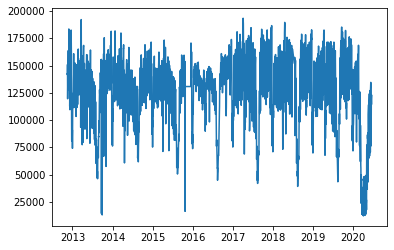
\includegraphics[width=0.75\textwidth]{trend_ingressi_areac}
\caption{Andamento del numero di ingressi in Area C registrati ai varchi}
\label{fig:trend_ingressi_areac}
\end{figure}

Nel grafico\ref{fig:trend_ingressi_areac} si nota come nel corso degli anni l'andamento del volume di traffico sia sempre stato piuttosto costante, mostrando un andamento ciclico caratterizzato da un calo, prevedibile, nei mesi estivi.
Si può chiaramente notare l'effetto lockdown, che ha portato ad avere il traffico a livelli molto più bassi di quanto mai visto in precedenza.
Nel corso degli anni, fatta eccezione per la particolare primavera di quest'anno, l'influenza del traffico sulle concentrazioni dovrebbe essere rimasta piuttosto invariata, anche se l'ammodernamento della flotta circolante potrebbe sicuramente aver ridotto le emissioni totali, anche a parità di numero di veicoli circolanti.

\subsection{$NO_x$}
Le prestazioni del modello ottenuto sono risultate in linea con quelle ottenute senza l'inclusione della variabile sul traffico. Questa misura, quindi, non ci permette di fare previsioni più precise di quanto non riuscissimo già a fare, ma ciò non significa che non ci possano essere delle differenze nelle serie normalizzate ottenute. 

Alla variabile è stata attribuita un'importanza di 0.07, la quinta maggiore tra le undici considerate, che significa che comunque un po' sia utilizzata per fare previsioni. L'importanza delle altre variabili del modello risulta invece praticamente invariata, con temperatura e velocità del vento che hanno continuato ad essere le due più importanti.

Uno strumento utile per verificare come il nostro modello utilizzi le variabili predittrici per fare previsioni sono i partial dependence plots. Questi grafici ci mostrano come vari il valore delle previsioni fatte dal nostro modello al variare del valore di una singola variabile, con tutte le altre fissate al loro valore medio.

\begin{figure}[h]
\centering
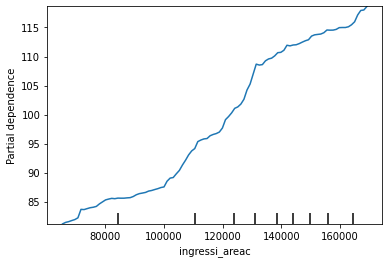
\includegraphics[width=0.75\textwidth]{nox_part_dep}
\caption{Partial dependence plot per il numero degli ingressi in Area C registrati ai varchi}
\label{fig:nox_part_dep}
\end{figure}

In figura\ref{fig:nox_part_dep} è riportato il partial dependence plot della variabile degli ingressi in Area C. Non sorprendentemente, visto il forte collegamento tra questi inquinanti ed il traffico, si vede come le previsioni del nostro modello arrivino ad avere valori decisamente maggiori al crescere del numero di ingressi registrati, con un aumento di oltre 30$\mu g/m^3$ se si raddoppia il numero di ingressi.

\begin{figure}[h]
\centering
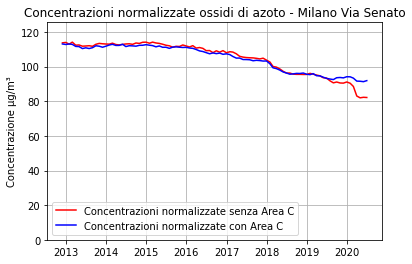
\includegraphics[width=0.75\textwidth]{nox_areac}
\caption{Confronto degli andamenti delle serie normalizzate ottenute usando o meno il numero di ingressi in Area C come variabile predittrice}
\label{fig:nox_areac}
\end{figure}

A primo impatto si nota subito come le due serie siano sempre praticamente equivalenti, mantenendo lo stesso andamento. Si nota anche, però, come per il 2020 le due serie mostrino andamenti molto diversi, con una differenza di circa 10 $\mu g/m^3$ sulle concentrazioni previste.
Come avevamo visto in precedenza è proprio nel 2020 che il traffico ha fatto registrare un importante calo, dovuto alle misure per il contenimento dei contagi da COVID, e si nota chiaramente come in corrispondenza di questo calo le previsioni dei due modelli siano discordanti.
Da un lato si vede come il modello costruito senza l'uso del numero di ingressi registrati in Area C abbia effettivamente rilevato un calo abbastanza importante nelle concentrazioni misurate, dovuto proprio alla diminuzione del traffico. Dall'altro si vede invece come il modello costruito usando anche i dataset di Area C non rilevi questa differenza, continuando a mantenere un andamento in linea col trend decrescente di questi ultimi anni. Questo modello, infatti, essendo stato costruito utilizzando anche i dati sul traffico è capace di eliminarne l'influenza (e ciò avviene sia in condizioni di traffico al di sopra che al di sotto della media) e rapportando i dati dei mesi della primavera 2020 a condizioni di traffico medie ha eliminato il calo rilevato in precedenza. Questo ci dà ulteriormente conferma dell'origine da attribuire a tale calo ed inoltre ci dà una stima di come mediamente potrebbero cambiare le concentrazioni se venisse completamente (o quasi, proprio come è successo nei mesi di lockdown) eliminato il traffico veicolare privato.

Per quanto riguarda gli $NO_x$ abbiamo quindi dimostrato come effettivamente anche i nostri modelli siano in grado di individuare l'influenza del traffico sulle concentrazioni e abbiamo provato anche a quantificare il possibile miglioramento della qualità dell'aria che si otterrebbe eliminandolo completamente.
Un'altra nota da fare è che i modelli creati utilizzando anche i dati degli ingressi in Area C individuano comunque lo stesso trend decrescente nelle concentrazioni già visto in precedenza, mostrandoci quindi come questo andamento non sia associabile al volume del traffico, ma che le sue cause siano da ricercare altrove. Questa è un'ulteriore conferma di come l'innovazione tecnologica sia il maggior responsabile del miglioramento delle concentrazioni di questo inquinante, oltre che al modo più efficace per la loro riduzione.

\subsection{$NO_2$}
Per completezza è stato trattato anche il biossido di azoto.

\begin{figure}[h]
\centering
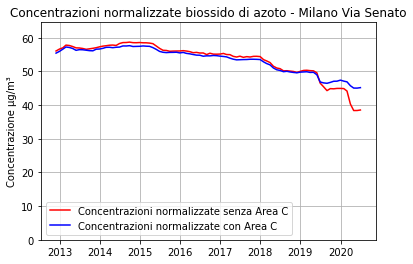
\includegraphics[width=0.75\textwidth]{no2_areac}
\caption{Confronto degli andamenti delle serie normalizzate ottenute usando o meno il numero di ingressi in Area C come variabile predittrice}
\label{fig:no2_areac}
\end{figure}

Anche per questo inquinante valgono le stesse considerazioni fatte per gli ossidi. Importante notare come anche questa volta ci sia una differenza di andamento per l'anno 2020 associabile proprio al calo del traffico circolante dovuto al lockdown.

\subsection{CO}
Le stesse prove, effettuate con la creazione di un modello per la trattazione che faccia uso anche del numero degli ingressi in Area C, sono state fatte sul monossido di carbonio.

\begin{figure}[h]
\centering
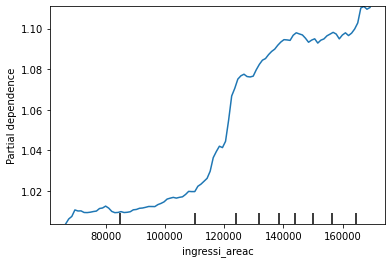
\includegraphics[width=0.75\textwidth]{co_part_dep}
\caption{Partial dependence plot per il numero degli ingressi in Area C registrati ai varchi}
\label{fig:co_part_dep}
\end{figure}

Anche se l'aumento rilevato al raddoppiare del traffico non è sicuramente consistente come quelli riguardanti gli ossidi di azoto, anche in questo caso possiamo notare come il nostro modello associ una crescita delle concentrazioni al crescere del traffico. 

%inserisci grafico
\begin{figure}[h]
\centering
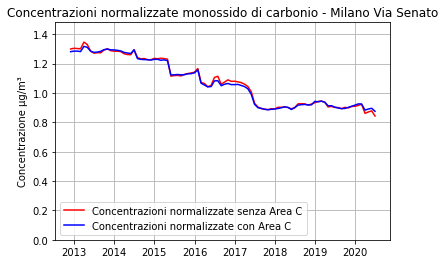
\includegraphics[width=0.75\textwidth]{co_areac}
\caption{Confronto degli andamenti delle serie normalizzate ottenute usando o meno il numero di ingressi in Area C come variabile predittrice}
\label{fig:co_areac}
\end{figure}

Guardando il grafico\ref{fig:co_areac} si nota nuovamente come le serie ottenute siano sempre piuttosto equivalenti. Ci sono due piccole discrepanze sui risultati ottenuti, una riguardante il periodo dell'epidemia di COVID ed una a cavallo tra gli anni 2016 e 2017.
Per il periodo riguardante l'epidemia di COVID si nota la stessa situazione vista per gli ossidi di azoto, con il modello costruito senza i dati di Area C che fa previsioni leggermente più basse rispetto all'altro, potenzialmente collegabili alla diminuzione del traffico. Per quanto riguarda il periodo tra il 2016 ed il 2017 si vede invece come le previsioni di tale modello siano più alte, come se l'influenza del traffico in tale periodo sia stata maggiore. Controllando il grafico del numero di ingressi visto in precedenza, però, non si notano aumenti nel numero di veicoli circolanti che possano giustificare tale differenza, quindi le cause potrebbero essere altre oppure si potrebbe semplicemente trattare di una differnza delle previsioni dei due modelli che comunque può esserci, trattandosi di previsioni basate su modelli statistici e che quindi hanno una certa variabilità.
Trattandosi comunque entrambe di diffrenze minime è difficile stabilire con certezza le cause che stanno alla loro origine.

Per il monossido di carbonio, quindi, l'influenza del traffico sembra essere davvero minima, anche perchè si sta comunque parlando di concentrazioni molto basse. L'innovazione tecnologica del mondo delle auto ha fatto sì che questo inquinante ormai non sia più un effettivo problema.

\subsection{PM10}
L'esperimento è stato ripetuto anche per le polveri sottili (in particolare il PM10 - per il PM2.5 si ha comunque una situazione praticamente analoga).

\begin{figure}[h]
\centering
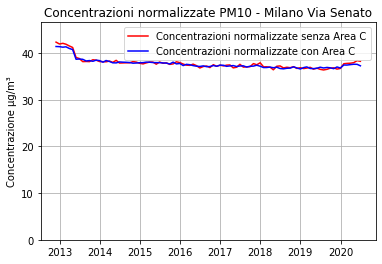
\includegraphics[width=0.75\textwidth]{pm10_areac}
\caption{Confronto degli andamenti delle serie normalizzate ottenute usando o meno il numero di ingressi in Area C come variabile predittrice}
\label{fig:pm10_areac}
\end{figure}

Vediamo infatti come le due serie rimangano praticamente sempre equivalenti, non mostrando particolari scostamenti neanche nel periodo dell'epidemia di COVID.

Per quanto riguarda le polveri sottili, quindi, il nostro metodo non rileva una particolare influenza dell'andamento del traffico sulle concentrazioni registrate, nemmeno a seguito di un calo del volume come quello che è avvenuto nel lockdown, mostrandoci ancora una volta come le fonti emissive più influenti per questi inquinanti non siano i veicoli a motore.

\chapter{Effetti del lockdown per il Covid-19 sulle concentrazioni degli inquinanti}
I mesi primaverili del 2020 sono stati caratterizzati dalla diffusione dell'epidemia di Covid-19 e dalle importanti misure prese per il suo contenimento. Queste limitazioni hanno portato ad avere un quadro emissivo eccezionale per gli inquinanti atmosferici, che difficilmente si sarebbe potuto verificare in condizioni normali. Questi mesi, infatti, sono stati caratterizzati da importanti limitazioni sugli spostamenti e alle attività produttive, quindi rappresentano un importante banco di prove per verificare come siano cambiate le concentrazioni degli inquinanti in atmosfera con una così drastica riduzione delle attività antropiche, dandoci la possibilità di valutare come effettivamente si potrebbe intervenire per ottenere ulteriori miglioramenti della qualità dell'aria.

L'obbiettivo delle nostre analisi è stato mettere alla prova la nostra tecnica di normalizzazione per vedere come siano effettivamente cambiate le concentrazioni degli inquinanti durante i mesi dell'epidemia rispetto agli anni precedenti, dopo aver eliminato la variabilità derivata dalle condizoni meteorologiche e stagionali. È infatti importante considerare che l'epidemia è arrivata durante dei mesi che già normalmente sono abbastanza favorevoli per la maggior parte degli inquinanti di interesse, poichè le condizioni atmosferiche e meteorologiche dei mesi primaverili portano sempre ad un abbassamento delle concentrazioni misurate rispetto ai mesi invernali.
Potendo eliminare la variabilità data dalla stagionalità e da queste condizioni meteorologiche che influenzano così tanto i valori misurati è quindi sicuramente interessante cercare di capire quanto i classici cali delle concentrazioni registrati nei mesi primaverili siano stati influenzati dal blocco generale avuto dalle attività umane in tali mesi.

Abbiamo quindi trattato tutti gli inquinanti, confrontando l'andamento dei mesi tra febbraio e maggio del 2020 con quello degli anni tra il 2015 e il 2019 della media delle serie, normalizzate e non, dei capoluoghi di provincia già usate per le analisi precedenti. In questo modo potremo verificare se per i mesi dell'epidemia il nostro modello ha rilevato dei cali riconducibili proprio alle limitazioni imposte, in modo da capire quale tipo di interventi possa risultare più efficacie per il contenimento delle concentrazioni di ciascuno.

\section{$NO_x$ e $NO_2$}
\subsection{$NO_x$}
Abbiamo iniziato le nostre analisi trattando gli ossidi di azoto che, viste le limitazioni agli spostamenti e considerato il loro collegamento con l'andamento del traffico, potrebbero essere potenzialmente gli inquinanti più colpiti durante questi mesi di lockdown. Ad influire, inoltre, potrebbe sicuramente essere stato anche il parziale calo delle emissioni industriali, dovuto al fermo delle attività non ritenute essenziali.

\begin{figure}[h]
\centering
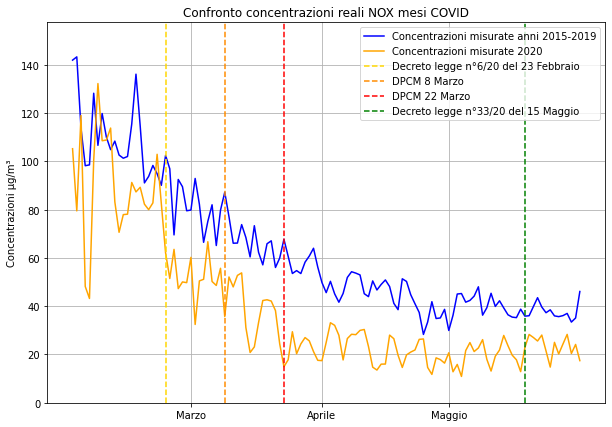
\includegraphics[width=0.75\textwidth]{nox_covid}
\caption{Confronto tra l'andamento della serie misurata del 2020 con la media di quelle degli anni 2015-2019}
\label{fig:nox_covid}
\end{figure}

\begin{figure}[h]
\centering
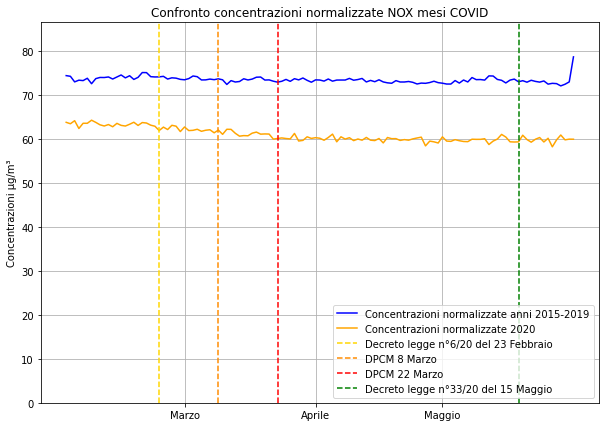
\includegraphics[width=0.75\textwidth]{nox_covid_norm}
\caption{Confronto tra l'andamento della serie normalizzata del 2020 con la media di quelle degli anni 2015-2019}
\label{fig:nox_covid_norm}
\end{figure}

Guardando il grafico delle concentrazioni misurate\ref{fig:nox_covid} si nota chiaramente il calo delle concentrazioni classico dei mesi primaverili, causato proprio dalle condizioni più favorevoli alla dispersione. Tale calo, chiaramente, risulta invece eliminato quando si considerano le serie normalizzate (grafico\ref{fig:nox_covid_norm}).
Guardando sia i grafici delle concentrazioni reali che quello delle serie normalizzate si osserva come nei mesi di lockdown le concentrazioni abbiano subito un importante ribasso rispetto agli anni precedenti, sicuramente dovuto al blocco del traffico e di alcune attività produttive. 

\subsection{$NO_2$}
Abbiamo verificato anche i dati relativi al biossido di azoto, aspettandoci comunque di ottenere risultati abbastanza simili a quelli visti sugli ossidi trattati nel loro complesso.

\begin{figure}[h]
\centering
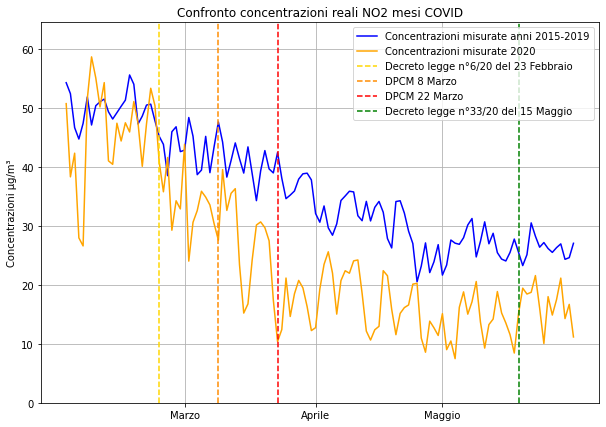
\includegraphics[width=0.75\textwidth]{no2_covid}
\caption{Confronto tra l'andamento della serie misurata del 2020 con la media di quelle degli anni 2015-2019}
\label{fig:no2_covid}
\end{figure}

\begin{figure}[h]
\centering
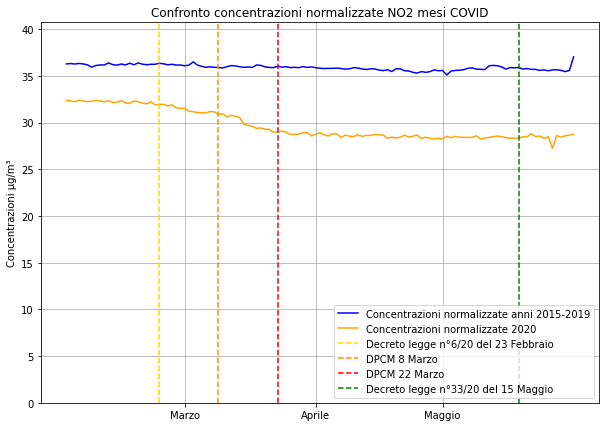
\includegraphics[width=0.75\textwidth]{no2_covid_norm}
\caption{Confronto tra l'andamento della serie normalizzata del 2020 con la media di quelle degli anni 2015-2019}
\label{fig:no2_covid_norm}
\end{figure}

Anche in questo caso, infatti, oltre al classico calo dei mesi primaverili, si vede una differenza tra le concentrazioni del 2020 e quelle degli anni precedenti, sia considerando le concentrazioni misurate che guardando le serie normalizzate.
Anche in questo caso le cause sono sicuramente da attribuire alle stesse ragioni che hanno portato al calo degli ossidi.

Chiaramente una misura così restrittiva non è sicuramente applicabile in modo continuo, ma ci dimostra come interventi su larga scala possano avere un discreto impatto sulle concentrazioni a differenza di quello che si era visto analizzando dei provvedimenti presi in particolari località, i cui effetti si sono rivelati minimi se non addirittura nulli.
Interventi su larga scala richiederebbero investimenti sull'innovazione tecnologica, per poter arrivare ad avere una flotta di veicoli circolanti a bassissime emissioni, così come potrebbe essere sicuramente utile investire su motorizzazioni "pulite" come quella elettrica. Chiaramente questo tipo di interventi richiede tempo, soprattutto per quanto riguarda i motori elettrici che al momento presentano ancora diverse problematiche da risolvere, e ci dimostra come non sia possibile intervenire sugli inquinanti pensando di abbatterne le concentrazioni rapidamente.

\section{PM10 e PM2.5}
Per quanto riguarda le polveri sottili e l'andamento delle concentrazioni nel periodo di lockdown la situazione risulta essere più complessa rispetto agli ossidi di azoto.
Se da un lato, infatti, i cali di traffico e produzione industriale hanno sicuramente portato ad un calo delle emissioni, dall'altro si è visto un aumento di quelle derivanti da riscaldamenti domestici, causato da un maggior fabbisognio giornaliero delle famiglie costrette a restare più tempo nell'abitazione a causa delle misure imposte. 

\begin{figure}[h]
\centering
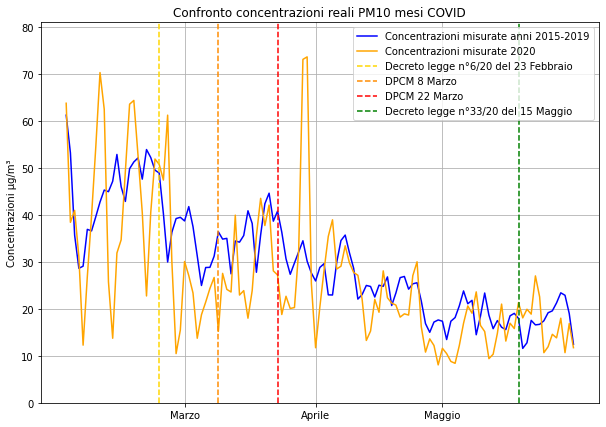
\includegraphics[width=0.75\textwidth]{pm10_covid}
\caption{Confronto tra l'andamento della serie misurata del 2020 con la media di quelle degli anni 2015-2019}
\label{fig:pm10_covid}
\end{figure}

\begin{figure}[h]
\centering
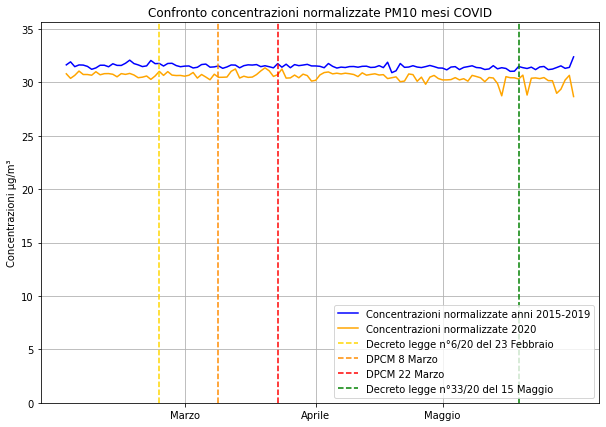
\includegraphics[width=0.75\textwidth]{pm10_covid_norm}
\caption{Confronto tra l'andamento della serie normalizzata del 2020 con la media di quelle degli anni 2015-2019}
\label{fig:pm10_covid_norm}
\end{figure}

Per quanto riguarda la frazione più spessa del particolato (PM10) vediamo come le concentrazioni misurate si mantengano piuttosto in linea con quanto visto negli anni precedenti, con episodi come quello di fine Marzo in cui le concentrazioni hanno fatto registrare valori ben al di sopra del limite di legge, nonostante fossero già in vigore tutte le limitazioni imposte coi vari DPCM per il contenimento dei contagi.
La serie normalizzata\ref{fig:pm10_covid_norm}, invece, evidenzia un leggero calo rispetto agli anni precedenti, che però potrebbe essere collegato al leggero trend decrescente che era già stato visto sulle serie normalizzate di questo inquinante.

\begin{figure}[h]
\centering
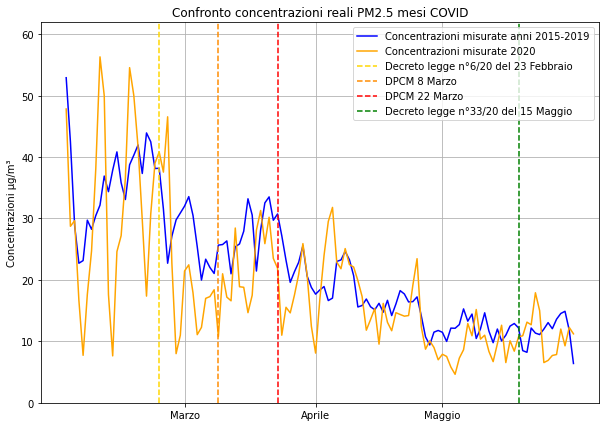
\includegraphics[width=0.75\textwidth]{pm25_covid}
\caption{Confronto tra l'andamento della serie misurata del 2020 con la media di quelle degli anni 2015-2019}
\label{fig:pm25_covid}
\end{figure}

\begin{figure}[h]
\centering
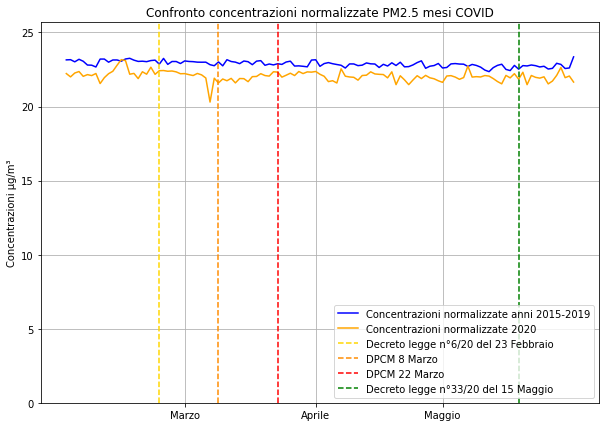
\includegraphics[width=0.75\textwidth]{pm25_covid_norm}
\caption{Confronto tra l'andamento della serie normalizzata del 2020 con la media di quelle degli anni 2015-2019}
\label{fig:pm25_covid_norm}
\end{figure}

Esattamente come visto in precedenza, anche per la frazione più fine di particolato le concentrazioni si mantengono abbastanza invariate rispetto agli anni precedenti, con una piccola discrepanza sulle serie normalizzate nuovamente dovuta alla presenza di un trend leggermente calante individuato per le serie normalizzate di questo inquinante\ref{fig:pm25_covid_norm}.

Per quanto riguarda il particolato, quindi, nonostante la riduzione del traffico e delle attività produttive, il maggior fabbisogno energetico delle famiglie ha fatto sì che le concentrazioni rimanessero comunque su livelli più o meno simili a quelli degli anni precedenti.
Questo ci mostra come effettivamente per trattare questi inquinanti, la cui origine è sicuramente varia e complessa, non si possano prendere provvedimenti riguardanti solamente un settore in particolare, come potrebbe essere il traffico, ma vanno pensati dei piani che riguardino tutte le fonti emissive.
La presenza di un trend negativo per tutte e due le frazioni di particolato è sicuramente un'indicazione che comunque la strada che si sta percorrendo negli ultimi anni sia quella giusta e che sia necessario proseguire investendo sempre di più su innovazione tecnologica e fonti rinnovabili.

\section{CO}
Anche per quanto riguarda il monossido di carbonio il quadro emissivo è cambiato durante i mesi dell'epidemia, con l'importante riduzione del traffico che però anche in questo caso è stata bilanciata dal maggior uso dei riscaldamenti domestici. Traffico e combustioni non industriali, infatti, sono le due categorie maggiormente responsabili delle emissioni di questo inquinante in atmosfera.

\begin{figure}[h]
\centering
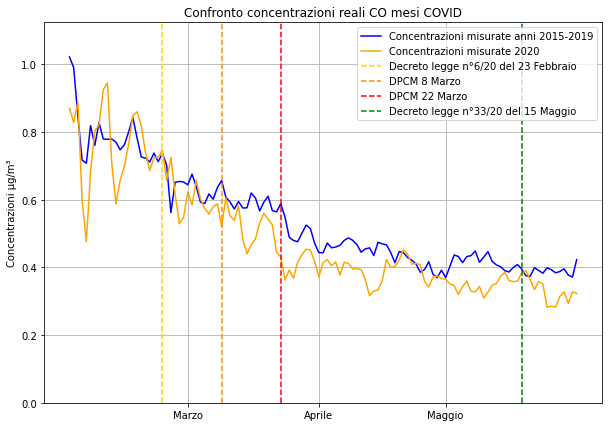
\includegraphics[width=0.75\textwidth]{co_covid}
\caption{Confronto tra l'andamento della serie misurata del 2020 con la media di quelle degli anni 2015-2019}
\label{fig:co_covid}
\end{figure}

\begin{figure}[h]
\centering
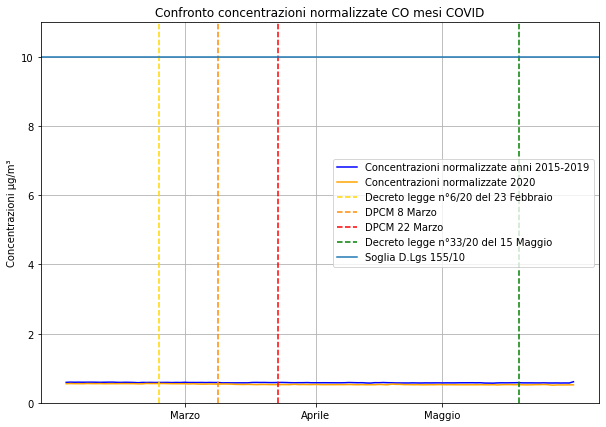
\includegraphics[width=0.75\textwidth]{co_covid_norm}
\caption{Confronto tra l'andamento della serie normalizzata del 2020 con la media di quelle degli anni 2015-2019}
\label{fig:co_covid_norm}
\end{figure}

Successivamente all'applicazione delle limitazioni tramite l'emanazione dei DPCM del mese di Marzo si nota come effettivamente le concentrazioni misurate di monossido di carbonio risultino essere leggermente minori rispetto a quelle degli anni precedenti\ref{fig:co_covid}. Tale differenza viene confermata anche dalle serie normalizzate, anche se bisogna ricordare che si tratta di differenze minime su valori già molto bassi.

Le limitazioni imposte, quindi, potrebbero aver avuto qualche effetto sulle concentrazioni di monossido di carbonio, anche se ormai la situazione per questo inquinante non risulta più essere così critica e quindi c'è anche meno interesse nella ricerca di nuove misure di contenimento, visto che quelle già presenti risultano essere più che sufficientemente efficaci.

\section{Benzene}
Il benzene è sicuramente un inquinante importante da analizzare in questo periodo, visto che spesso viene indicato come tracciante del traffico veicolare (specialmente quello motorizzato a benzina) che proprio in questi mesi ha subito importanti limitazioni e potrebbe quindi aver portato ad un calo delle concentrazioni misurate.

\begin{figure}[h]
\centering
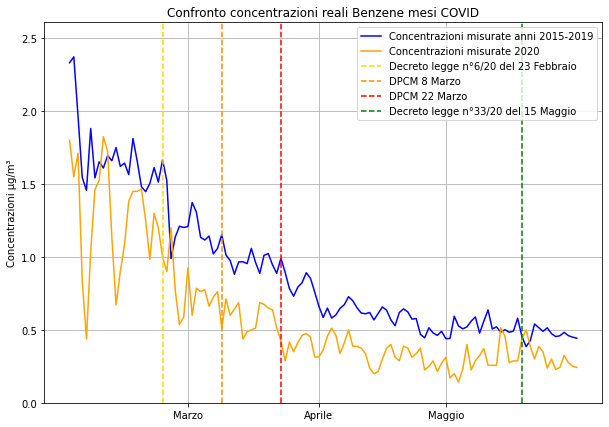
\includegraphics[width=0.75\textwidth]{benzene_covid}
\caption{Confronto tra l'andamento della serie misurata del 2020 con la media di quelle degli anni 2015-2019}
\label{fig:benzene_covid}
\end{figure}

\begin{figure}[h]
\centering
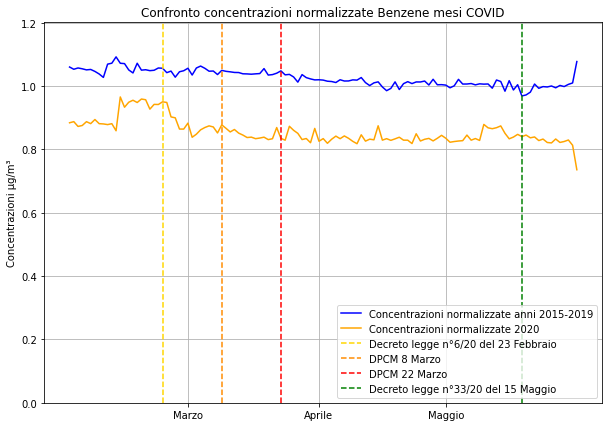
\includegraphics[width=0.75\textwidth]{benzene_covid_norm}
\caption{Confronto tra l'andamento della serie normalizzata del 2020 con la media di quelle degli anni 2015-2019}
\label{fig:benzene_covid_norm}
\end{figure}

Anche per questo inquinante, così collegato al traffico, notiamo uno scostamento rispetto all'andamento degli anni precedenti abbastanza comptabile con quello visto sugli ossidi di azoto.
Questo scostamento, confermato anche dalle serie normalizzate, conferma come effettivamente il traffico influenzi le concentrazioni di questo inquinante e quindi come una sua riduzione abbia conseguentemente portato ad un abbassamento delle concentrazioni.

Sebbene la situazione per quanto riguarda il benzene non desti preoccupazioni, visto che i livelli ormai sono ampiamente sotto alle soglie di legge, abbiamo visto come una riduzione del traffico abbia portato ad un ulteriore miglioramento della situazione per quanto riguarda questo inquinante, che è auspicabile venga portato avanti dall'innovazione tecnologica nel corso dei prossimi anni.

\section{SO2}
Analizziamo l'andamento delle concentrazioni di biossido di zolfo durante i mesi di lockdown, per vedere se notiamo differenze rispetto agli anni precedenti, pur ricordando che si sta trattando un inquinante le cui concentrazioni sono ormai prossime al fondo naturale.

\begin{figure}[h]
\centering
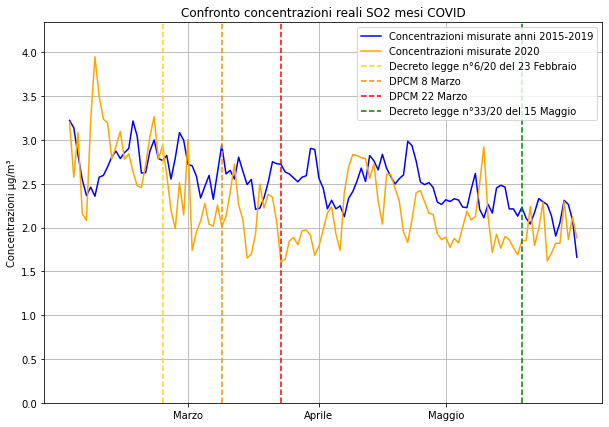
\includegraphics[width=0.75\textwidth]{so2_covid}
\caption{Confronto tra l'andamento della serie misurata del 2020 con la media di quelle degli anni 2015-2019}
\label{fig:so2_covid}
\end{figure}

\begin{figure}[h]
\centering
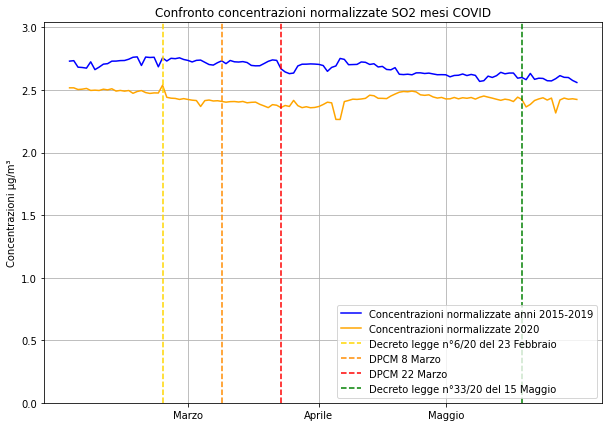
\includegraphics[width=0.75\textwidth]{so2_covid_norm}
\caption{Confronto tra l'andamento della serie normalizzata del 2020 con la media di quelle degli anni 2015-2019}
\label{fig:so2_covid_norm}
\end{figure}

Si vede infatti come le concentrazioni si siano mantenute su un livello praticamente in linea con quello degli anni precedenti e come anche le serie normalizzate siano piuttosto simili, anche se per il 2020 risulta effettivamente esserci stato un leggero calo, di cui però, vista la modesta quantità, è difficile stabilire se sia dovuto alle limitazioni imposte durante il lockdown o se la sua origine sia anche dovuta ad altri fattori (come ad esempio fluttuazioni nel fondo naturale).

\section{Ozono}
L'ozono, essendo un inquinante secondario, ha origine molto varie e quindi può essere interessante valutare quali siano state le concentrazioni registrate a seguito dei provvedimenti di lockdown. 

\begin{figure}[h]
\centering
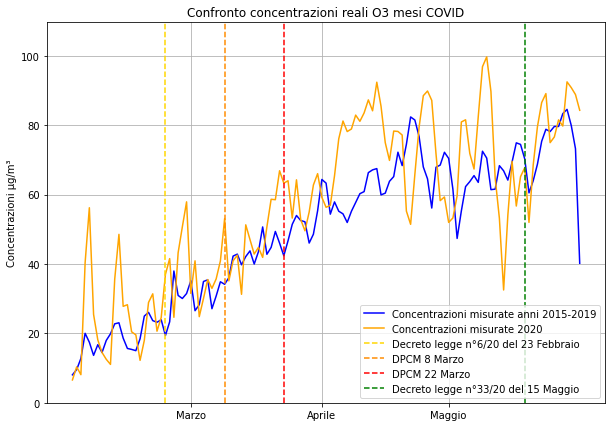
\includegraphics[width=0.75\textwidth]{o3_covid}
\caption{Confronto tra l'andamento della serie misurata del 2020 con la media di quelle degli anni 2015-2019}
\label{fig:o3_covid}
\end{figure}

\begin{figure}[h]
\centering
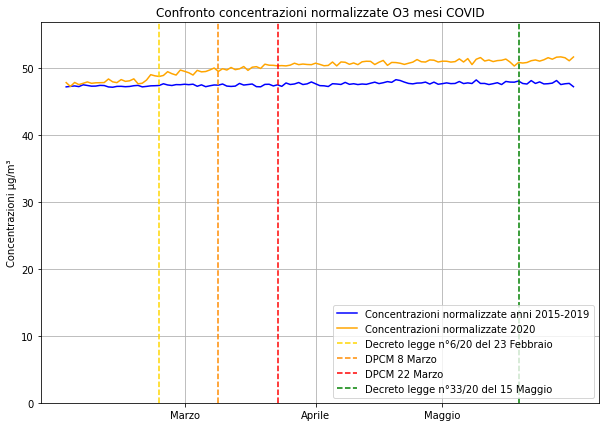
\includegraphics[width=0.75\textwidth]{o3_covid_norm}
\caption{Confronto tra l'andamento della serie normalizzata del 2020 con la media di quelle degli anni 2015-2019}
\label{fig:o3_covid_norm}
\end{figure}

Vediamo come le concentrazioni per quest'anno si siano mantenute abbastanza in linea con quelle degli anni precedenti mostrando il classico trend crescente dei mesi primaverili che caratterizza questo inquinante, con la serie normalizzata che segnala un aumento, dovuto probabilmente anche alla presenza del trend positivo già visto in precedenza.

Nonostante i grossi cambiamenti visti nei mesi di lockdown, quindi, l'ozono non risulta essere stato colpito da tali misure. Questo inquinante, considerate le sue complesse e varie origini, risulta quindi difficile da trattare e trovare misure per il suo contenimento è molto complesso. Si è comunque visto come un blocco generale delle attività non sia stato sufficiente per migliorarne la situazione.

\section{Ammoniaca}
In ultimo andiamo a controllare l'andamento dell'ammoniaca, per la quale le serie normalizzate dei nostri modelli avevano individuato un andamento piuttosto fluttuante.

\begin{figure}[h]
\centering
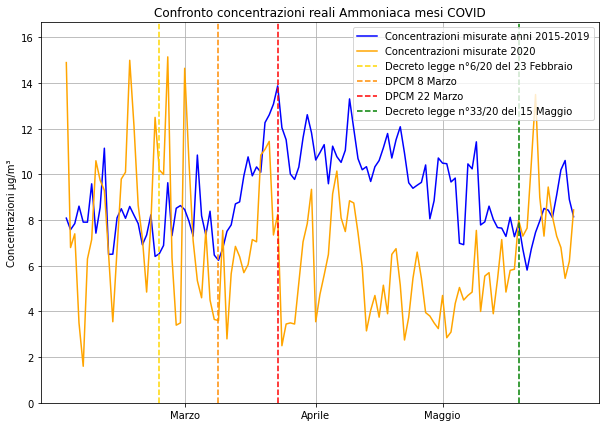
\includegraphics[width=0.75\textwidth]{ammoniaca_covid}
\caption{Confronto tra l'andamento della serie misurata del 2020 con la media di quelle degli anni 2015-2019}
\label{fig:ammoniaca_covid}
\end{figure}

\begin{figure}[h]
\centering
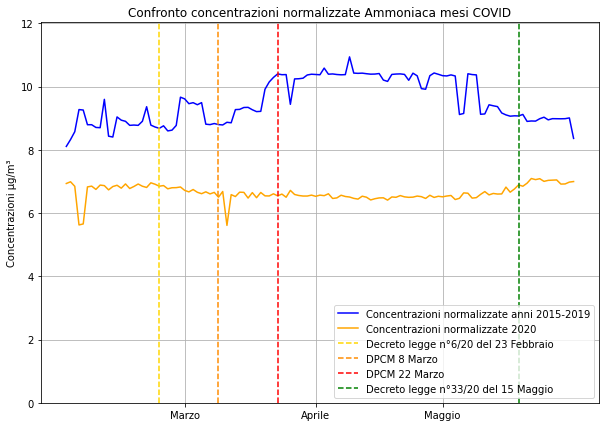
\includegraphics[width=0.75\textwidth]{ammoniaca_covid_norm}
\caption{Confronto tra l'andamento della serie normalizzata del 2020 con la media di quelle degli anni 2015-2019}
\label{fig:ammoniaca_covid_norm}
\end{figure}

Effettivamente controllando le concentrazioni misurate si note come tra Marzo e Maggio si sia visto un effettivo calo dei valori misurati, individuato anche dalle serie normalizzate.
Questo calo probabilmente deriva da una minor attività anche per quanto riguarda il settore agricolo, che è praticamente l'unico responsabile delle concentrazioni misurate di questo inuqinante, che è stato costretto a rallentare durante i mesi di lockdown.

Visto il forte collegamento tra questo inquinante e l'agricoltura qualsiasi misura di contenimento delle concentrazioni dovrà necessariamente agire su tale settore, poichè effettivamente con un calo dell'attività si è notato anche un calo nelle concentrazioni rilevate.

\chapter{Conclusioni}
Nelle nostre analisi abbiamo dimostrato come sia possibile applicare l'algoritmo Random Forest per eliminare l'influenza della meteorologia dalle serie dei principali inquinanti atmosferici, in modo da poterne analizzare l'andamento e le variazioni in modo più preciso.  
Controllare l'influenza della meteorologia in analisi di questo tipo è fondamentale, poichè la sua influenza risulta per la maggior parte delle volte essere maggiore di quella che possono avere limitazioni o particolari eventi che possono modificare le concentrazioni di inquinanti presenti in atmosfera. Random Forest, così come molte altre tecniche del mondo del machine learning, si adattano perfettamente a questo tipo di modellazione e permettono di ottenere dei risultati validi ed affidabili.  
Applicando la nostra tecnica per ottenere la normalizzazione meteorologica ai dati raccolti sul territorio della Regione Lombardia si è visto come ormai l'inquinamento atmosferico non sia più un problema grave, con la maggior parte degli inquinanti che sono ormai stabilmente sotto ai livelli classificati come pericolosi per la salute, fatta eccezione per ossidi di azoto e polveri sottili che non occasionalmente fanno registrare picci sopra ai livelli consigliati. Spesso comunque, come si capisce guardando gli andamenti delle serie normalizzate che sono stabili sotto alle soglie legislative attuali, questi superamenti sono causati da condizioni atmosferiche sfavorevoli che portano all'accumulo degli inquinanti in atmosfera piuttosto che a reali aumenti di emissioni antropiche.  
Il trend decrescente presente per molti inquinanti ci mostra come effettivamente il progresso tecnologico degli ultimi anni sia fondamentale per la riduzione dell'inquinamento e come questa sia probabilmente l'unica soluzione per quegli inquinanti che ancora oggi si mantengono su livelli più proeccupanti.  
Riguardo all'impatto del traffico sull'inquinamento si è visto come provvedimenti presi solo localmente, come possono essere state Area C o Area B per il comune di Milano, siano praticamente ininfluenti sia a causa del fatto che gli inquinanti in atmosfera possono viaggiare anche diversi chilometri che perchè ormai l'influenza del traffico, grazie alle numerose innovazioni introdotte nel corso degli anni. è piuttosto contenuta. Normalizzando le serie anche utilizzando i dati del traffico si è infatti visto come mediamente il suo apporto non porti a grosse variazioni sui valori registrati, se non durante il periodo del lockdown in cui si sono visti dei cali sulle concentrazioni di quegli inquinanti maggiormente collegati al traffico. L'entità di questi cali, comunque abbastanza contenuti, ci ha dimostrato come per il livello di tecnologia attuale effettivamente il contributo del traffico sia ormai abbastanza contenuto e questo non dovrebbe sorprenderci visti i sempre più stringenti limiti emissivi che vengono imposti.  
Occupandoci del priodo di lockdown primaverile causato dall'epidemia di Covid-19 non si sono riscontrate grosse variazioni rispetto alla situazione normale, poichè i cali nelle emissioni dovuti alla sospensione di alcune attività sono stati bilanciati dal maggior fabbisogno energetico delle famiglie. Solo per quanto riguarda gli inquinanti maggiormente collegati al traffico, ovvero ossidi di azoto e benzene, si sono visti dei cali di lieve entità compatibili con la riduzione del numero di veicoli circolanti. 

\bibliographystyle{plain}
\bibliography{Biblio}
%\addcontentsline{toc}{chapter}{Bibliografia}

\listoffigures

\end{document}
